\documentclass[12pt,a4paper]{article}

% TeX Gyre Termes is metrically identical to Times New Roman. Load it by file
% rather than by name: tectonic ships the font files but does not expose them
% to fontspec's system-font lookup.
\usepackage{fontspec}
\setmainfont{texgyretermes}[
  Extension      = .otf,
  UprightFont    = *-regular,
  BoldFont       = *-bold,
  ItalicFont     = *-italic,
  BoldItalicFont = *-bolditalic ]
\usepackage[a4paper,margin=2.5cm]{geometry}
\usepackage{graphicx}
\usepackage{booktabs}
\usepackage{longtable}
\usepackage{calc}
\providecommand{\real}[1]{#1}
\usepackage{array}
\usepackage{caption}
\usepackage{lineno}
\usepackage{textcomp}
\usepackage{microtype}
\usepackage{float}
\usepackage[hidelinks]{hyperref}
\usepackage{fancyhdr}
\usepackage{parskip}

% Frontiers asks for continuous line numbering and page numbers for review.
\usepackage{etoolbox}
\linenumbers
% lineno and longtable are mutually incompatible ("No counter 'none' defined"),
% so suspend numbering for the duration of each table.
\AtBeginEnvironment{longtable}{\nolinenumbers}
\AtEndEnvironment{longtable}{\linenumbers}
\pagestyle{fancy}
\fancyhf{}
\fancyfoot[C]{\thepage}
\renewcommand{\headrulewidth}{0pt}

% The figures are large; without these LaTeX defers every one of them to the
% end of the document rather than placing it near the text that discusses it.
\renewcommand{\topfraction}{0.92}
\renewcommand{\bottomfraction}{0.85}
\renewcommand{\textfraction}{0.06}
\renewcommand{\floatpagefraction}{0.72}
\setcounter{topnumber}{3}
\setcounter{bottomnumber}{2}
\setcounter{totalnumber}{5}

% Numeric tables are tight; stop TeX hyphenating tool names like MRtrix3
% across lines inside a cell, and give the columns a little more room.
\setlength{\tabcolsep}{4pt}

\captionsetup{font=small,labelfont=bf,justification=justified,
              singlelinecheck=false,skip=6pt}
\setcounter{secnumdepth}{0}
\setlength{\parindent}{0pt}
\linespread{1.05}

% pandoc emits \tightlist for compact lists
\providecommand{\tightlist}{%
  \setlength{\itemsep}{0pt}\setlength{\parskip}{0pt}}

% Verbatim inside tables needs a breakable column type
\newcolumntype{L}[1]{>{\raggedright\arraybackslash}p{#1}}

\title{\vspace{-2.2cm}\bfseries dMRI Rosetta Stone: An Open-Source Interactive
Platform for Cross-Tool Diffusion MRI Education and Reproducibility}
\author{Busra Mutlu\thanks{Correspondence: Busra Mutlu,
\texttt{[email address]}, Department of Neuroimaging, King's College London,
De Crespigny Park, London SE5 8AF, United Kingdom.}\\[2pt]
\normalsize Department of Neuroimaging, King's College London,
London, United Kingdom}
\date{}

\begin{document}
\maketitle
\thispagestyle{fancy}

\noindent\textbf{Article type:} Technology and Code \\
\textbf{Journal:} Frontiers in Neuroinformatics \\
\textbf{Specialty section:} Methods in Neuroimaging \\
\textbf{Running title:} dMRI Rosetta Stone: Cross-Tool dMRI Education Platform

\vspace{4pt}\hrule\vspace{10pt}

\section{Abstract}\label{abstract}

Diffusion MRI analysis is dominated by three software packages --- FSL, MRtrix3, and DIPY --- whose divergent command syntax, terminology, and algorithmic implementations create a substantial barrier for researchers learning, reproducing, or cross-validating analyses across ecosystems. No existing resource allows all three to be executed side by side on the same human brain data in one interface. We present dMRI Rosetta Stone, an open-source Streamlit platform, containerised with Docker, covering seven canonical pipeline stages: brain extraction, Marchenko-Pastur denoising, eddy and motion correction, tensor fitting, constrained spherical deconvolution, tractography, and voxelwise group analysis. At each stage the exact executable command for all three toolkits is displayed, run on open data, and its output rendered for direct comparison, with the asymmetries between toolkits made explicit rather than glossed over. Alongside the platform we report a reproducible benchmark of inter-tool agreement on two independent open datasets, Stanford HARDI and Sherbrooke 3-shell, driving all three toolkits from identical input volumes, gradient tables, and one shared brain mask so that the comparison isolates the tensor-fitting stage. Brain masks overlapped at Dice coefficients of 0.90 to 0.97 despite mask volumes differing by up to 21\%. Scalar agreement was strongly asymmetric, and the asymmetry replicated across both acquisitions: MRtrix3 and DIPY were near-identical in white matter (fractional anisotropy r = 0.9990 and 0.9966; mean diffusivity r = 0.9965 and 0.9991), whereas FSL diverged from both. Critically, the FSL discrepancy was not a fixed bias correctable by a scaling factor: mean diffusivity was consistently lower, but by 5\% on one dataset and 19\% on the other, and the anisotropy offset reversed sign between acquisitions. We further show that non-physical tensor fits, arising from unconstrained least squares, occurred in up to 4.0\% of white matter voxels in FSL and 2.0\% in MRtrix3 but never in DIPY, and that leaving them in place depresses an apparent diffusivity correlation from 0.997 to 0.118 --- a trap for anyone computing agreement statistics on raw diffusion maps. The container requires no local neuroimaging installation and runs on Linux, macOS, and Windows. dMRI Rosetta Stone is freely available at https://github.com/happybrotherhood/dmri-rosetta-stone under an MIT licence.

\textbf{Keywords:} diffusion MRI; FSL; MRtrix3; DIPY; educational software; neuroinformatics; reproducibility; open science

\section{Introduction}\label{introduction}

Diffusion magnetic resonance imaging (dMRI) is the principal non-invasive technique for probing white matter microstructure and structural connectivity in the living human brain (Basser et al., 1994; Jones, 2010). By encoding the directional displacement of water molecules, dMRI provides access to biophysical indices --- including fibre orientation, axon density, and myelin integrity --- that are invisible to conventional anatomical MRI (Beaulieu, 2002). Applications span fundamental neuroscientific questions about brain organisation and inter-individual variability, as well as clinical contexts including the characterisation of white matter alterations in neurodegenerative diseases, psychiatric conditions, and neurodevelopmental disorders (Catani and Thiebaut de Schotten, 2008; Jones, 2010).

The dMRI analysis ecosystem is dominated by three major software packages. FSL (FMRIB Software Library), developed at the University of Oxford, provides robust preprocessing, DTI fitting, and voxelwise group analysis via the Tract-Based Spatial Statistics (TBSS) pipeline (Smith et al., 2004; Jenkinson et al., 2012). MRtrix3, developed at The Florey Institute of Neuroscience and Mental Health, specialises in constrained spherical deconvolution (CSD) and high-fidelity fibre orientation modelling (Tournier et al., 2019). DIPY (Diffusion Imaging in Python) offers a flexible, Python-native implementation of the full dMRI pipeline and is widely used when algorithmic transparency or custom extensions are required (Garyfallidis et al., 2014).

Despite their complementary strengths, these toolkits present a significant practical barrier. Each employs distinct command-line syntax, file format conventions, and --- in several cases --- different terminology for the same operation. For example, brain extraction is called \texttt{bet} in FSL, \texttt{dwi2mask} in MRtrix3, and \texttt{median\_otsu} in DIPY. Mean diffusivity is reported as \texttt{MD} in FSL, \texttt{ADC} in MRtrix3, and \texttt{md} in DIPY. These surface-level differences cause genuine confusion for researchers trained in one ecosystem who attempt to read, reproduce, or extend work conducted in another.

A more substantive concern is methodological reproducibility. Published dMRI studies rarely justify their choice of software, and it is not always clear whether reported group differences in white matter metrics reflect genuine biological effects or implementation-level differences between tools (Bhagwat et al., 2021; Richie-Halford et al., 2022). Software-specific choices --- brain masking algorithm, denoising method, tensor fitting algorithm --- can introduce non-trivial variability in derived metrics such as fractional anisotropy (FA) and mean diffusivity (MD).

Existing educational resources address individual toolkits in depth. FSL is covered through the annual FSL Course and its wiki; MRtrix3 provides extensive documentation at docs.mrtrix.org; DIPY provides executable Jupyter notebook tutorials at dipy.org; Andy's Brain Book (Jahn, 2020) covers FSL comprehensively and touches on MRtrix3. However, no existing resource places all three toolkits side by side on the same data, in the same interface, with executable commands and live visual outputs. The specific combination of cross-tool coverage, real human brain data, browser-based executability, and zero neuroimaging software installation has not been offered by any prior platform (Table 2). This is the gap that dMRI Rosetta Stone addresses.

The name is drawn from the original Rosetta Stone (196 BCE), a priestly decree inscribed in three scripts --- Ancient Egyptian hieroglyphs, Demotic, and Ancient Greek --- whose parallel presentation enabled decipherment of a language unreadable for over a millennium. Here, FSL, MRtrix3, and DIPY are three parallel ``languages'' for dMRI analysis, and juxtaposing them enables translation between ecosystems.

\section{Design Principles}\label{design-principles}

Four principles guided development. First, \textbf{parallel transparency}: every pipeline stage must show the complete, executable command in all three toolkits simultaneously, without requiring the user to navigate between separate documents or websites. Second, \textbf{real human data}: the platform must operate on real brain acquisitions, not synthetic phantoms, because the noise, artefacts, and masking ambiguities that motivate each preprocessing step are only apparent on real data. Third, \textbf{zero installation barrier}: a researcher with no prior Linux or FSL experience should be able to run the full pipeline within minutes; this mandates containerisation of FSL, MRtrix3, and DIPY into a single portable image. Fourth, \textbf{conceptual scaffolding}: every stage must include a biological and mathematical explanation of what the operation does, why it is necessary, and when one toolkit should be preferred over another.

\section{Materials and Methods}\label{materials-and-methods}

\subsection{Software Availability and Requirements}\label{software-availability-and-requirements}

\begin{table}[htbp]
\centering\footnotesize
\hyphenpenalty=10000\exhyphenpenalty=10000\relax
\begin{tabular}{@{}
  >{\raggedright\arraybackslash}p{(\linewidth - 2\tabcolsep) * \real{0.5000}}
  >{\raggedright\arraybackslash}p{(\linewidth - 2\tabcolsep) * \real{0.5000}}@{}}
\toprule

\bottomrule

\textbf{Project name} & dMRI Rosetta Stone \\
\textbf{Project home page} & https://github.com/happybrotherhood/dmri-rosetta-stone \\
\textbf{Archived version} & v1.0.0, Zenodo, doi:10.5281/zenodo.22106455 (all versions: doi:10.5281/zenodo.22106454) \\
\textbf{Operating system} & Platform independent --- Linux, macOS, and Windows, via Docker \\
\textbf{Programming language} & Python $\geq$ 3.9 \\
\textbf{Other requirements} & Docker $\geq$ 20.10. For local installation without Docker: FSL $\geq$ 6.0 and MRtrix3 $\geq$ 3.0.4 \\
\textbf{Bundled toolkits} & FSL 6.0.7, MRtrix3 3.0.4, DIPY $\geq$ 1.7 \\
\textbf{Licence} & MIT \\
\textbf{Restrictions for non-academic use} & None imposed by this project. Note, however, that the bundled FSL is distributed under the FSL Licence, which restricts commercial use; users intending commercial deployment must obtain a licence from Oxford University Innovation. MRtrix3 (MPL 2.0) and DIPY (BSD 3-clause) carry no such restriction. \\
\end{tabular}
\end{table}

\subsection{Software Architecture}\label{software-architecture}

dMRI Rosetta Stone is implemented as a Streamlit web application (version $\geq$ 1.40; Streamlit Inc., 2019) and containerised with Docker (Merkel, 2014). Streamlit converts Python scripts into interactive browser-based interfaces without requiring HTML, CSS, or JavaScript, making the codebase accessible to any researcher with Python familiarity.

The Dockerfile uses a two-stage build (Figure 1). Stage 1 copies MRtrix3 3.0.4 binaries from the official \texttt{mrtrix3/mrtrix3:latest} image. Stage 2 starts from \texttt{ubuntu:22.04}, installs FSL 6.0.7 via the official \texttt{fslinstaller.py} script, copies MRtrix3 from Stage 1, and installs the Python stack --- Streamlit, DIPY $\geq$ 1.7, nibabel, numpy, scipy, matplotlib, pandas, scikit-image --- via pip. This multi-stage approach avoids dependency conflicts between FSL and MRtrix3 that arise from single-stage installation. The container serves the Streamlit interface at \texttt{http://localhost:8501} via two commands:

\begin{verbatim}
docker build --platform linux/amd64 -t dmri-rosetta .
docker run --rm --platform linux/amd64 -p 8501:7860 dmri-rosetta
\end{verbatim}

The first command builds the image (approximately 15 minutes, dominated by the FSL download); the second launches the container. No neuroimaging software is required on the host machine.


\begin{figure}[tbp]
  \centering
  \setcounter{figure}{0}
  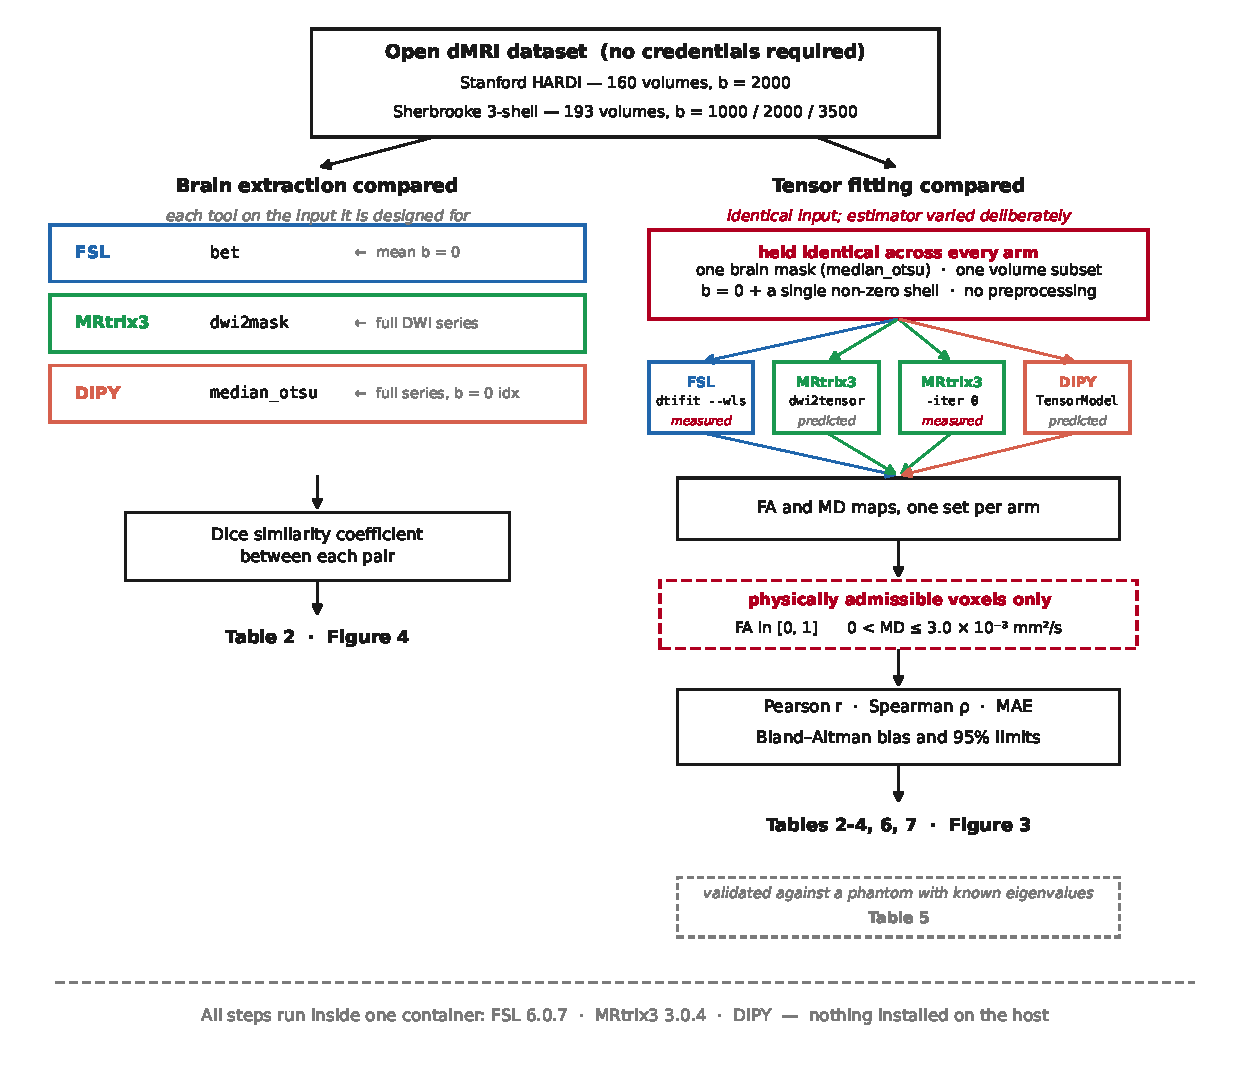
\includegraphics[width=1.0\textwidth]{figures/Figure1.pdf}
  \caption{Software architecture of the dMRI Rosetta Stone Docker container. \emph{Build time (top):} a two-stage build copies MRtrix3 3.0.4 binaries from the official \texttt{mrtrix3/mrtrix3} image into an \texttt{ubuntu:22.04} stage that installs FSL 6.0.7 via \texttt{fslinstaller.py} and the Python stack (Streamlit, DIPY, nibabel, numpy, scipy, matplotlib) via pip. Separating the two avoids the dependency conflicts that arise when FSL and MRtrix3 are installed into a single stage. \emph{Run time (bottom):} the user reaches the Streamlit application through a browser on port 8501, and the application dispatches pipeline commands to all three toolkits via Python \texttt{subprocess} inside the container. Open sample data is mounted from the host. No neuroimaging software is installed on the host machine. The diagram is generated by \texttt{scripts/make\_fig1\_architecture.py}.}
  \label{fig:Figure1}
\end{figure}



\subsection{Data}\label{data}

All demonstrations use the Stanford HARDI dataset distributed by the DIPY project under an open-access licence (Rokem et al., 2015). The dataset comprises 160 volumes (10 b = 0, 150 DWI at b = 2000 s/mm\textsuperscript{2}) with voxel size 2 $\times$ 2 $\times$ 2 mm and matrix 81 $\times$ 106 $\times$ 76. It is downloaded automatically on first launch via DIPY's \texttt{get\_fnames("stanford\_hardi")} utility without credentials. A brain mask is generated at download time using \texttt{median\_otsu} and stored alongside the raw NIfTI data.

The quantitative benchmark reported below additionally uses the Sherbrooke 3-shell dataset, distributed openly as part of the DIPY sample data collection (Garyfallidis et al., 2014) and retrieved via \texttt{get\_fnames("sherbrooke\_3shell")}; like the Stanford data it requires no credentials. It comprises 193 volumes (1 b = 0; 64 directions at each of b = 1000, 2000, and 3500 s/mm\textsuperscript{2}) with voxel size 2 $\times$ 2 $\times$ 2 mm and matrix 128 $\times$ 128 $\times$ 60. The dataset is distributed with DIPY rather than accompanied by a dedicated acquisition publication, and we use it here as an independent test acquisition rather than as a characterised reference sample. Because it differs from the Stanford data in site, protocol, angular sampling, b-value range, and --- importantly for the results below --- the number of b = 0 volumes, analysing both provides an independent replication of the inter-tool comparison rather than a second look at one acquisition.

The application also supports Human Connectome Project (HCP; Van Essen et al., 2013) multi-shell data (b = 1000/2000/3000 s/mm\textsuperscript{2}, 90 directions per shell) for users with HCP data access credentials, enabling demonstration of multi-tissue CSD which requires multiple non-zero b-value shells.

\subsection{Pipeline Coverage}\label{pipeline-coverage}

The application covers seven pipeline stages, each as a dedicated page in the sidebar navigation (Table 1).

\textbf{Brain Extraction.} FSL \texttt{bet}, MRtrix3 \texttt{dwi2mask}, and DIPY \texttt{median\_otsu} are demonstrated on the same b = 0 volume. Outputs are displayed as a red-tinted mask overlay on the b = 0 image (Figure 4).

\textbf{Denoising (MP-PCA).} Marchenko-Pastur PCA exploits diffusion signal redundancy to separate signal from thermal noise using random matrix theory (Veraart et al., 2016). MRtrix3 \texttt{dwidenoise} and DIPY \texttt{mppca} are demonstrated. FSL lacks a dedicated denoising tool; this asymmetry is made explicit with an explanation of when denoising is most beneficial.

\textbf{Eddy Current and Motion Correction.} FSL \texttt{eddy\_cpu} (Andersson and Sotiropoulos, 2016), MRtrix3 \texttt{dwifslpreproc} (which wraps FSL eddy internally and prepends Gibbs-ringing removal via \texttt{mrdegibbs}), and DIPY \texttt{motion\_correction} (rigid-body registration only, no eddy correction) are demonstrated. A demo subsample mode (5 b = 0 + 15 DWI volumes) reduces runtime from approximately 40 minutes to approximately 3 minutes for interactive use.

\textbf{DTI Fitting.} FSL \texttt{dtifit}, MRtrix3 \texttt{dwi2tensor} + \texttt{tensor2metric}, and DIPY \texttt{TensorModel.fit()} are applied to the same input data; FA, MD, AD, and RD maps are rendered for each toolkit (Figure 3).

\textbf{Constrained Spherical Deconvolution.} MRtrix3 \texttt{dwi2fod} (single-shell CSD, Tournier et al., 2007; multi-shell multi-tissue CSD, Jeurissen et al., 2014) and DIPY \texttt{ConstrainedSphericalDeconvModel} are demonstrated. FSL does not include CSD; its omission is discussed together with acquisition requirements for CSD ($\geq$ 30 directions, high b-value).

\textbf{Tractography.} MRtrix3 \texttt{tckgen} with the iFOD2 probabilistic algorithm (Tournier et al., 2010) and streamline filtering via \texttt{tcksift2} (Smith et al., 2015), FSL \texttt{probtrackx2} (command display and conceptual overview), and DIPY \texttt{LocalTracking} (deterministic, DTI peaks) are demonstrated. Track density images (TDI) generated with \texttt{tckmap} provide voxelwise streamline density maps.

\textbf{TBSS Voxelwise Group Analysis.} The full TBSS pipeline (Smith et al., 2006) --- \texttt{tbss\_1\_preproc}, \texttt{tbss\_2\_reg}, \texttt{tbss\_3\_postreg}, \texttt{tbss\_4\_prestats}, and \texttt{randomise} --- is demonstrated. Because the platform operates on a single subject, a synthetic group is constructed by adding Gaussian noise realisations ($\sigma$ = 0.03 FA units) to the real FA map. The absence of equivalent voxelwise pipelines in MRtrix3 and DIPY (fixel-based analysis in MRtrix3 is noted as the conceptual analogue) is made explicit.

\subsection{Concepts and Reference Module}\label{concepts-and-reference-module}

A dedicated Reference section provides: (1) a DTI metrics guide with the biological interpretation of FA, MD, AD, and RD and live map display; (2) a 16-term dMRI glossary; (3) a command cheat sheet covering all seven stages across all three toolkits; and (4) a decision framework for selecting the appropriate toolkit based on acquisition type, research question, and available compute resources.

\subsection{Quantitative Inter-Tool Agreement Analysis}\label{quantitative-inter-tool-agreement-analysis}

Beyond the interactive pipeline, we conducted a systematic quantitative comparison of DTI scalar metrics and brain masks across all three toolkits, on both the Stanford HARDI and the Sherbrooke 3-shell datasets. This analysis serves two purposes: it validates that the platform produces outputs consistent with established diffusion MRI principles, and it constitutes a reproducible, openly available benchmark of inter-tool agreement under controlled conditions --- identical input volumes, identical gradient tables, and a single shared brain mask.

\textbf{Brain mask agreement} was assessed using the Dice similarity coefficient (DSC) between each pair of binary masks produced by FSL \texttt{bet}, MRtrix3 \texttt{dwi2mask}, and DIPY \texttt{median\_otsu}. Each tool was run in its own idiomatic configuration rather than forced onto a common input, because the input a tool is designed to consume is part of the algorithm being compared: \texttt{bet} operates on the mean b = 0 image, \texttt{dwi2mask} on the full DWI series, and \texttt{median\_otsu} on the full series with the b = 0 volumes indexed. The DSC therefore quantifies the end-to-end difference between the three brain-extraction routines as a user would actually invoke them. DSC values are reported in Table 3.

Separately, and to keep brain extraction from confounding the metric comparison, a \emph{single} shared brain mask generated by \texttt{median\_otsu} was supplied to all three tensor fits. A white matter reference mask, defined as voxels where all three tools jointly yielded FA \textgreater{} 0.2, was used for all subsequent metric comparisons.

\textbf{DTI metric agreement} was assessed for FA and MD on both datasets. To isolate tensor-fitting differences from every other source of variability, all three tools were applied to the \emph{identical} input: the same unprocessed volumes, the same bvals and bvecs, and the shared \texttt{median\_otsu} brain mask described above. No denoising or eddy-current correction was applied before fitting. This omission is deliberate rather than a shortcut: any preprocessing step would itself be a toolkit-specific choice, and applying one tool's preprocessing to all three would confound the very comparison it is meant to enable. The consequence, which we state plainly, is that the reported agreement characterises the tensor-fitting stage alone and not a complete analysis pipeline.

For the multi-shell Sherbrooke data a further step was required. The single-tensor model assumes monoexponential signal decay, which does not hold across shells; FSL \texttt{dtifit} and MRtrix3 \texttt{dwi2tensor} silently fit every volume they are given, whereas DIPY requires the shell to be selected by the user. Left unaddressed, the three toolkits would have fitted different data and any difference between them would confound tensor fitting with shell selection. We therefore extracted the b = 0 and b = 1000 s/mm\textsuperscript{2} volumes (65 of 193) once, and passed that identical subset to all three toolkits. The Stanford data is single-shell, so all 160 volumes were used.

Voxelwise Pearson correlation coefficients (r), Spearman rank correlations ($\rho$), and mean absolute error (MAE) were computed over white matter voxels, and Bland--Altman analysis was performed for each cross-tool pair to characterise the distribution of voxelwise differences and identify any systematic bias.

Statistics were restricted to voxels whose values are physically admissible in both tools of a given pair: FA within {[}0, 1{]}, and MD positive and no greater than the diffusivity of free water at body temperature (3.0 $\times$ $10^{-3}$ mm\textsuperscript{2}/s). This restriction is necessary rather than cosmetic. Unconstrained linear tensor fitting can return negative eigenvalues, which drive FA above unity and MD below zero; because Pearson correlation is dominated by extreme values, a few hundred such voxels are sufficient to depress the apparent MD agreement from r = 0.997 to r = 0.118 while changing the mean absolute error by less than 2\%. The per-tool counts of these non-physical voxels are reported in the Results as a substantive inter-tool difference in their own right.

Results are reported in Tables 3 and 4 and in Figures 3 and 4, with the corresponding Sherbrooke figures provided as Supplementary Figures S1 and S2. All analyses were performed using the companion scripts \texttt{scripts/generate\_fa\_maps.py} and \texttt{scripts/compute\_fa\_comparison.py} distributed with the repository. Every value reported here is reproducible from openly available data with no credentials, by running:

\begin{verbatim}
python scripts/generate_fa_maps.py      --subject stanford
python scripts/compute_fa_comparison.py --subject stanford
python scripts/generate_fa_maps.py      --subject sherbrooke --shell 1000
python scripts/compute_fa_comparison.py --subject sherbrooke
\end{verbatim}

\section{Results}\label{results}

\subsection{Brain Mask Agreement}\label{brain-mask-agreement}

Brain masks produced by FSL \texttt{bet}, MRtrix3 \texttt{dwi2mask}, and DIPY \texttt{median\_otsu}, each run on the input its algorithm is designed to consume, showed high pairwise overlap on both datasets (Table 3). Dice similarity coefficients ranged from 0.9009 to 0.9277 on Stanford and from 0.9058 to 0.9668 on Sherbrooke, with no pair falling below 0.90 in either acquisition.

Pairwise Dice, however, conceals how differently the three algorithms behave, and it conceals it in a way worth making explicit to learners: for a large, compact object such as the brain, DSC stays high even when boundary decisions differ appreciably. On Stanford the mask volumes were 203,984 voxels (FSL), 187,948 (DIPY), and 167,950 (MRtrix3) --- a spread of 21\% between the largest and the smallest, despite every pairwise DSC exceeding 0.90. Nor is the ordering stable across acquisitions. On Sherbrooke the volumes were 199,249 (MRtrix3), 188,717 (FSL), and 186,450 (DIPY), a spread of only 7\%, with MRtrix3 moving from the most conservative mask on one dataset to the most inclusive on the other. Which tool yields the largest brain mask is therefore a property of the tool \emph{and} the acquisition together, not of the tool alone.

Disagreements were concentrated at the cortical boundary and, distinctively, at the lateral ventricles (Figure 4). DIPY \texttt{median\_otsu} excluded ventricular CSF, whereas FSL \texttt{bet} and MRtrix3 \texttt{dwi2mask} retained it. This reflects both the different tissue models each algorithm employs --- Otsu intensity thresholding after median filtering in DIPY, a deformable surface model in FSL \texttt{bet}, signal averaging over the DWI series in MRtrix3 \texttt{dwi2mask} --- and the different inputs those models are designed to consume, which is part of what distinguishes them in practice. The consequence is practical rather than cosmetic: a mask that includes ventricles admits high-diffusivity, near-isotropic voxels into any subsequent group statistics. These differences are displayed in Figure 4 and annotated in the Stage 1 interface.


\begin{figure}[tbp]
  \centering
  \setcounter{figure}{3}
  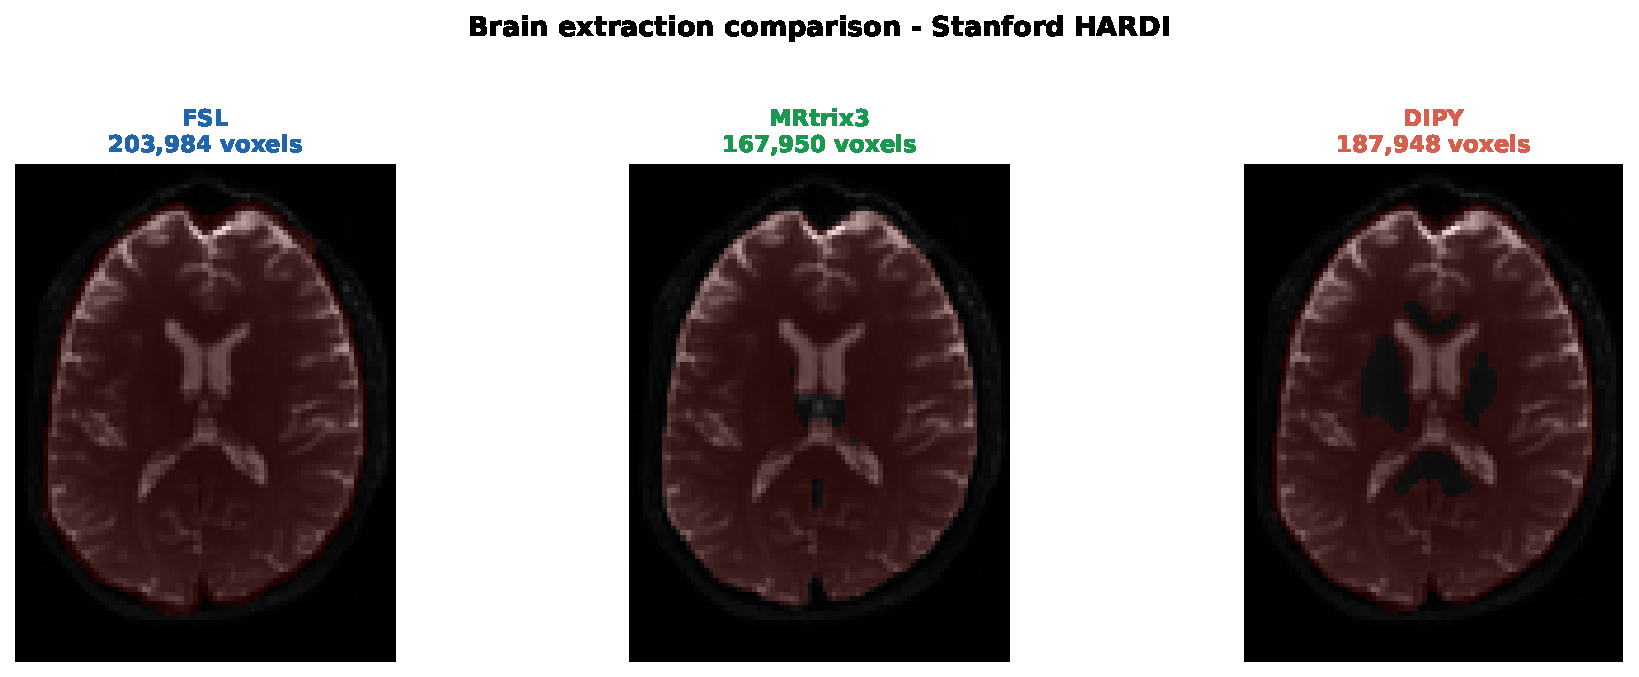
\includegraphics[width=1.0\textwidth]{figures/Figure4.pdf}
  \caption{Brain extraction comparison on the Stanford HARDI dataset (the Sherbrooke equivalent is provided as Supplementary Figure S2). The b = 0 mean image (greyscale) with brain mask overlaid in red, produced by FSL \texttt{bet} (left, 203,984 voxels), MRtrix3 \texttt{dwi2mask} (centre, 167,950 voxels), and DIPY \texttt{median\_otsu} (right, 187,948 voxels) from the same input volume. Dice similarity coefficients for each pair are reported in Table 3. Two differences are visible: the extent of cortical boundary coverage, and the treatment of the lateral ventricles, which DIPY \texttt{median\_otsu} excludes while FSL \texttt{bet} and MRtrix3 \texttt{dwi2mask} retain. These reflect the distinct tissue models employed by each algorithm.}
  \label{fig:Figure4}
\end{figure}



\subsection{Inter-Tool DTI Metric Agreement}\label{inter-tool-dti-metric-agreement}

\begin{table}[H]
\caption*{\textbf{Table 3. Quantitative inter-tool agreement for brain masks and DTI scalar metrics, on two independent open datasets.} Brain mask agreement assessed by Dice similarity coefficient (DSC) between each pair of per-tool brain extractions. DTI metric agreement assessed over white matter voxels (FA \textgreater{} 0.2 in all three tools) by Pearson correlation coefficient (r), mean absolute error (MAE), Bland--Altman mean bias, and 95\% limits of agreement (LoA). All three tensor fits used the same shared brain mask and the same volume subset, so metric differences reflect tensor fitting rather than masking or shell selection. MD in \textmu{}m\textsuperscript{2}/ms. Statistics are restricted to voxels physically admissible in both tools of the pair (FA $\in$ {[}0, 1{]}; 0 \textless{} MD $\leq$ 3.0 $\times$ $10^{-3}$ mm\textsuperscript{2}/s).}
\emph{Stanford HARDI (single shell, b = 2000 s/mm\textsuperscript{2}, 160 volumes; n = 65,002 white matter voxels)}\par\smallskip
\centering\footnotesize
\hyphenpenalty=10000\exhyphenpenalty=10000\relax
\begin{tabular}{@{}
  >{\raggedright\arraybackslash}p{(\linewidth - 14\tabcolsep) * \real{0.1250}}
  >{\raggedright\arraybackslash}p{(\linewidth - 14\tabcolsep) * \real{0.1250}}
  >{\raggedright\arraybackslash}p{(\linewidth - 14\tabcolsep) * \real{0.1250}}
  >{\raggedright\arraybackslash}p{(\linewidth - 14\tabcolsep) * \real{0.1250}}
  >{\raggedright\arraybackslash}p{(\linewidth - 14\tabcolsep) * \real{0.1250}}
  >{\raggedright\arraybackslash}p{(\linewidth - 14\tabcolsep) * \real{0.1250}}
  >{\raggedright\arraybackslash}p{(\linewidth - 14\tabcolsep) * \real{0.1250}}
  >{\raggedright\arraybackslash}p{(\linewidth - 14\tabcolsep) * \real{0.1250}}@{}}
\toprule
\begin{minipage}[b]{\linewidth}\raggedright
Comparison
\end{minipage} & \begin{minipage}[b]{\linewidth}\raggedright
Mask DSC
\end{minipage} & \begin{minipage}[b]{\linewidth}\raggedright
FA r
\end{minipage} & \begin{minipage}[b]{\linewidth}\raggedright
FA MAE
\end{minipage} & \begin{minipage}[b]{\linewidth}\raggedright
FA bias
\end{minipage} & \begin{minipage}[b]{\linewidth}\raggedright
FA 95\% LoA
\end{minipage} & \begin{minipage}[b]{\linewidth}\raggedright
MD r
\end{minipage} & \begin{minipage}[b]{\linewidth}\raggedright
MD MAE
\end{minipage} \\
\midrule

\bottomrule

FSL vs.~DIPY & 0.9277 & 0.9604 & 0.0228 & $-$0.0158 & {[}$-$0.0992, +0.0676{]} & 0.9368 & 0.0325 \\
FSL vs.~MRtrix3 & 0.9024 & 0.9652 & 0.0247 & $-$0.0181 & {[}$-$0.0964, +0.0602{]} & 0.9402 & 0.0333 \\
MRtrix3 vs.~DIPY & 0.9009 & 0.9990 & 0.0029 & +0.0027 & {[}$-$0.0107, +0.0162{]} & 0.9965 & 0.0012 \\
\end{tabular}
\end{table}

\emph{Sherbrooke 3-shell (b = 0 + b = 1000 s/mm\textsuperscript{2} subset, 65 volumes; n = 111,032 white matter voxels)}

\begin{table}[htbp]
\centering\footnotesize
\hyphenpenalty=10000\exhyphenpenalty=10000\relax
\begin{tabular}{@{}
  >{\raggedright\arraybackslash}p{(\linewidth - 14\tabcolsep) * \real{0.1250}}
  >{\raggedright\arraybackslash}p{(\linewidth - 14\tabcolsep) * \real{0.1250}}
  >{\raggedright\arraybackslash}p{(\linewidth - 14\tabcolsep) * \real{0.1250}}
  >{\raggedright\arraybackslash}p{(\linewidth - 14\tabcolsep) * \real{0.1250}}
  >{\raggedright\arraybackslash}p{(\linewidth - 14\tabcolsep) * \real{0.1250}}
  >{\raggedright\arraybackslash}p{(\linewidth - 14\tabcolsep) * \real{0.1250}}
  >{\raggedright\arraybackslash}p{(\linewidth - 14\tabcolsep) * \real{0.1250}}
  >{\raggedright\arraybackslash}p{(\linewidth - 14\tabcolsep) * \real{0.1250}}@{}}
\toprule
\begin{minipage}[b]{\linewidth}\raggedright
Comparison
\end{minipage} & \begin{minipage}[b]{\linewidth}\raggedright
Mask DSC
\end{minipage} & \begin{minipage}[b]{\linewidth}\raggedright
FA r
\end{minipage} & \begin{minipage}[b]{\linewidth}\raggedright
FA MAE
\end{minipage} & \begin{minipage}[b]{\linewidth}\raggedright
FA bias
\end{minipage} & \begin{minipage}[b]{\linewidth}\raggedright
FA 95\% LoA
\end{minipage} & \begin{minipage}[b]{\linewidth}\raggedright
MD r
\end{minipage} & \begin{minipage}[b]{\linewidth}\raggedright
MD MAE
\end{minipage} \\
\midrule

\bottomrule

FSL vs.~DIPY & 0.9668 & 0.8897 & 0.0504 & +0.0148 & {[}$-$0.1640, +0.1937{]} & 0.9012 & 0.1272 \\
FSL vs.~MRtrix3 & 0.9058 & 0.9157 & 0.0460 & +0.0139 & {[}$-$0.1419, +0.1696{]} & 0.9020 & 0.1271 \\
MRtrix3 vs.~DIPY & 0.9163 & 0.9966 & 0.0059 & +0.0053 & {[}$-$0.0260, +0.0366{]} & 0.9991 & 0.0029 \\
\end{tabular}
\end{table}

All three tools produced visually consistent FA maps (Figure 3a), with the canonical high-FA signature (FA \textgreater{} 0.6) in compact white matter tracts --- corpus callosum, corticospinal tract, superior longitudinal fasciculus --- and low FA values (FA \textless{} 0.2) in grey matter and CSF. On the Stanford data, mean white matter FA was 0.4000 $\pm$ 0.1479 (FSL), 0.4182 $\pm$ 0.1532 (MRtrix3), and 0.4168 $\pm$ 0.1537 (DIPY), with mean MD of 0.6034 $\pm$ 0.1295, 0.6350 $\pm$ 0.1442, and 0.6334 $\pm$ 0.1460 \textmu{}m\textsuperscript{2}/ms respectively. On the Sherbrooke data the corresponding values were FA 0.4775 $\pm$ 0.1977, 0.4698 $\pm$ 0.1914, and 0.4741 $\pm$ 0.1978, and MD 0.5224 $\pm$ 0.2249, 0.6410 $\pm$ 0.2820, and 0.6388 $\pm$ 0.2814 \textmu{}m\textsuperscript{2}/ms. All lie within the range conventionally reported for healthy white matter.

These per-tool means are computed over each tool's own physically admissible voxels, whereas the Bland--Altman bias in Table 3 is computed over voxels admissible in \emph{both} tools of a pair. The two therefore need not agree exactly, and on Sherbrooke --- where the number of excluded voxels differs substantially between toolkits --- they do not: the FSL-minus-MRtrix3 difference in means is +0.0077 FA units against a paired bias of +0.0139. The paired statistic is the appropriate one for agreement, since it compares the same voxels in both tools.

The comparison does not, however, partition symmetrically across the three toolkits, and the asymmetry takes the same form on both datasets.

\textbf{MRtrix3 and DIPY are near-identical.} On Stanford, FA agreement reached r = 0.9990 (Spearman $\rho$ = 0.9997, MAE = 0.0029, LoA {[}$-$0.0107, +0.0162{]}) and MD agreement r = 0.9965 (MAE = 0.0012 \textmu{}m\textsuperscript{2}/ms). On Sherbrooke the corresponding values were r = 0.9966 for FA and r = 0.9991 for MD. Differences of this magnitude are an order of magnitude below within-tract biological variability (FA SD $\approx$ 0.05--0.10) and are of no practical consequence in either acquisition.

\textbf{FSL is the outlier of the three, on both datasets.} Its agreement with the other two was consistently and substantially lower: FA r = 0.9652 and 0.9604 on Stanford, falling to 0.9157 and 0.8897 on Sherbrooke; MD r = 0.9402 and 0.9368 on Stanford, and 0.9020 and 0.9012 on Sherbrooke. Bland--Altman analysis (Figure 3c) showed systematic bias rather than symmetric scatter in every FSL pairing, and the limits of agreement against FSL --- roughly $\pm$0.08 FA units on Stanford and $\pm$0.17 on Sherbrooke --- reach or exceed the scale of within-tract biological variability.

\textbf{The direction of the offset, however, does not replicate for FA.} Mean diffusivity behaved consistently: FSL returned lower MD than both other toolkits on both datasets, by 0.033 \textmu{}m\textsuperscript{2}/ms on Stanford (approximately 5\%) and by 0.127 \textmu{}m\textsuperscript{2}/ms on Sherbrooke (approximately 19\%). Fractional anisotropy did not. On Stanford, FSL FA was \emph{lower} than MRtrix3 and DIPY by 0.018 and 0.016 units; on Sherbrooke it was \emph{higher}, by 0.014 and 0.015. The sign of the FA discrepancy reverses between acquisitions, and its magnitude changes by a factor of four for MD.

This is a more consequential finding than a fixed offset would have been. A constant bias, once characterised, can in principle be corrected or absorbed into a covariate. A bias whose sign depends on the acquisition cannot: there is no single correction factor to apply, and an analyst comparing FA values across studies processed with different software has no way to anticipate even the direction of the discrepancy. Because all three fits were driven from identical input data, identical gradient tables, one shared brain mask, and one shared volume subset, the effect must originate in the tensor-fitting stage itself. All three toolkits were run with weighted linear least squares, but their weighting schemes, regularisation, and outlier handling differ in implementation, and the interaction between those choices and acquisition properties such as b-value, SNR, and the number of b = 0 volumes is evidently not negligible. We report this as an empirical observation across two acquisitions; identifying the precise algorithmic mechanism would require a controlled comparison of the fitting routines themselves, which lies beyond the scope of this platform paper.


\begin{figure}[tbp]
  \centering
  \setcounter{figure}{2}
  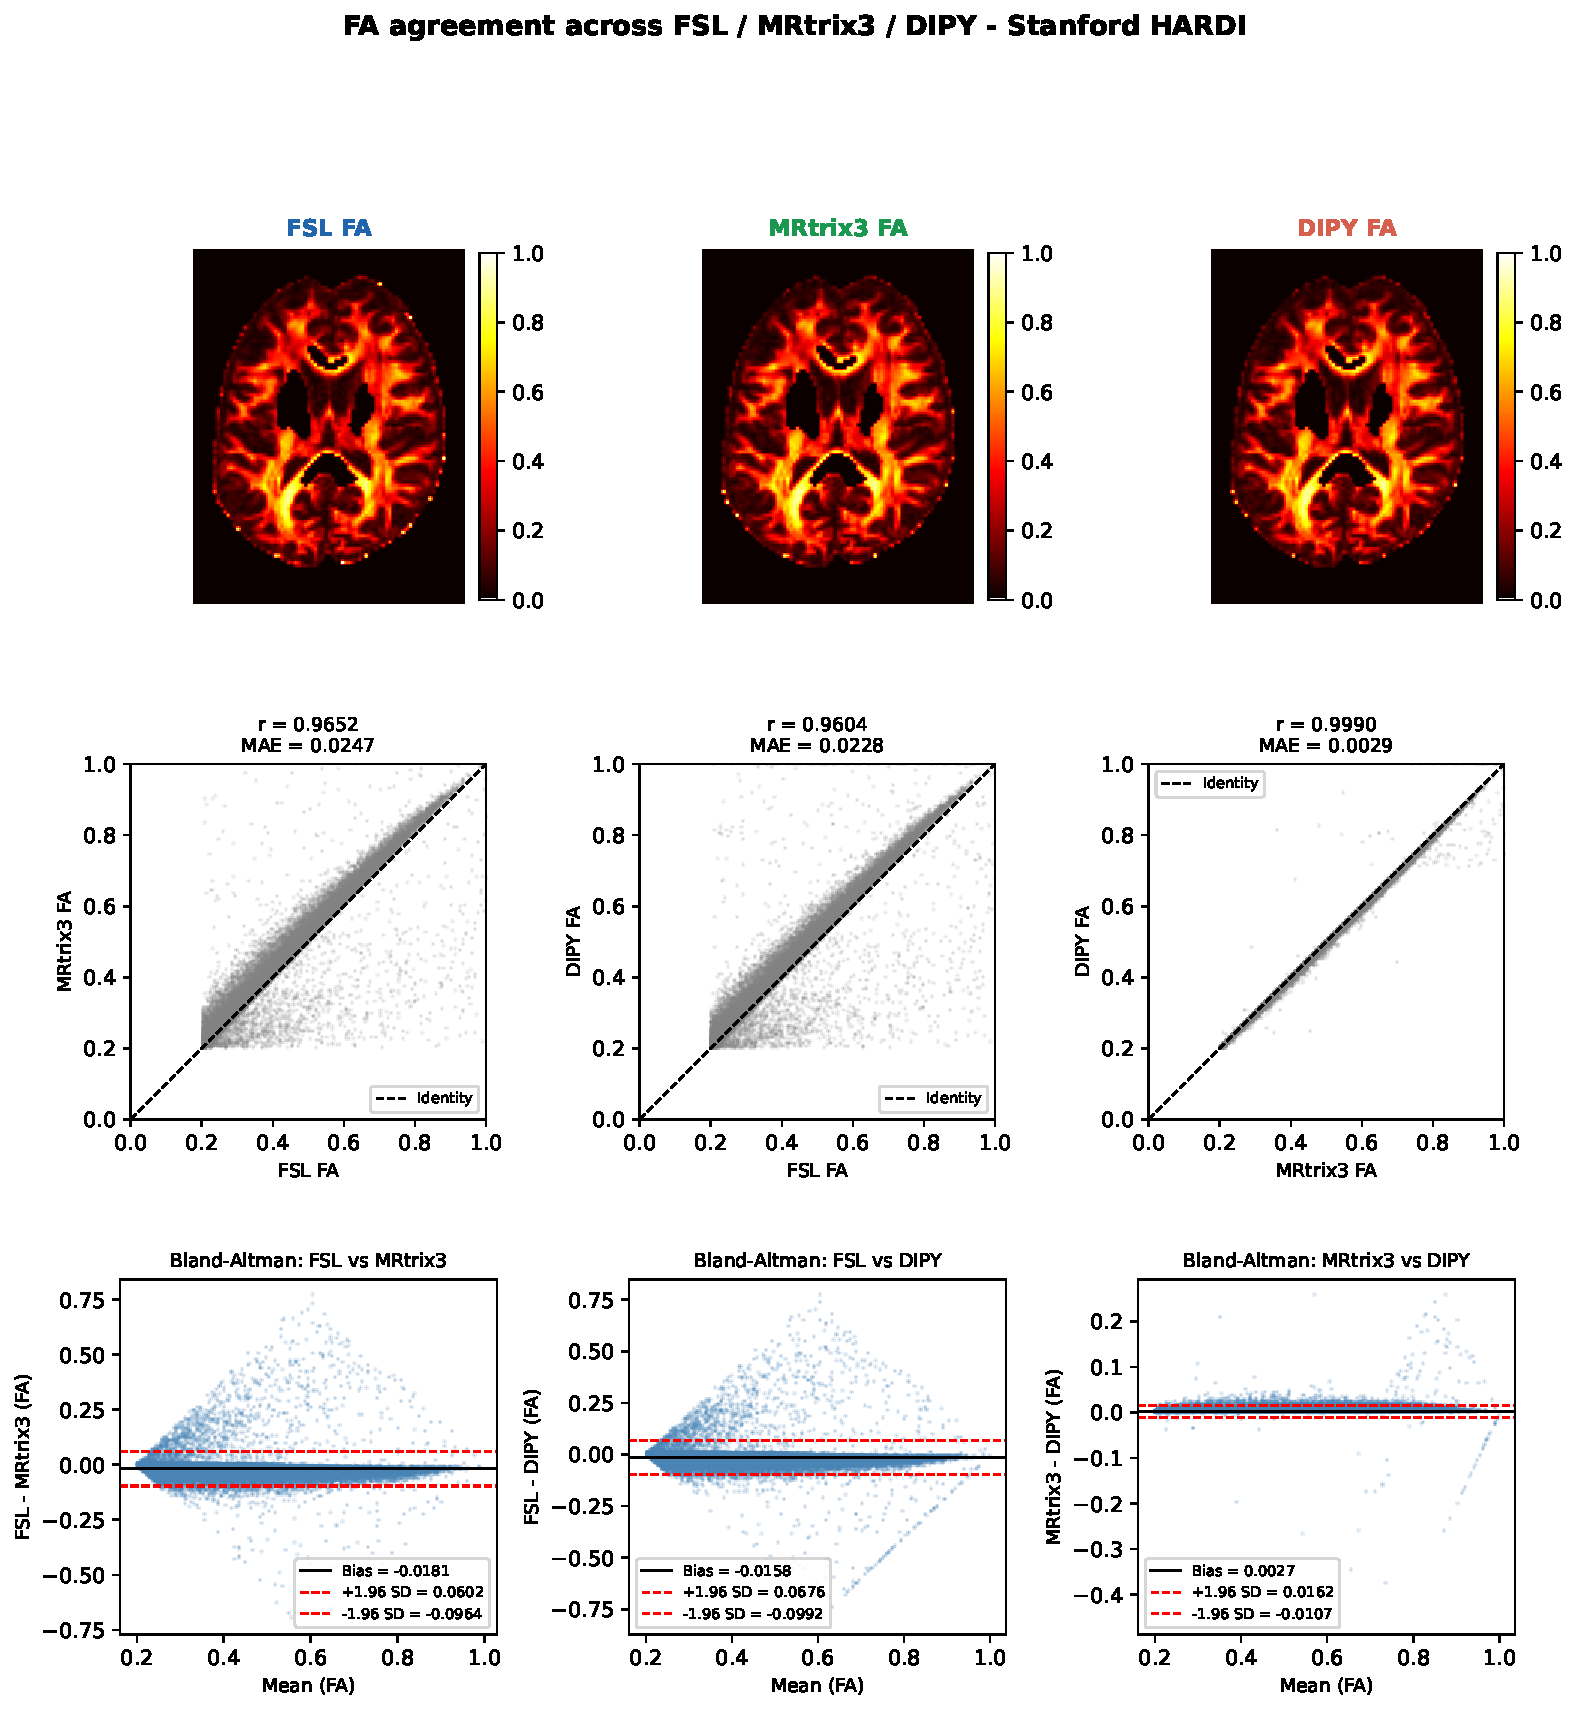
\includegraphics[width=0.86\textwidth]{figures/Figure3.pdf}
  \caption{Quantitative inter-tool DTI metric agreement, shown for the Stanford HARDI dataset (the equivalent panel for Sherbrooke 3-shell is provided as Supplementary Figure S1; both are generated by the same script). \textbf{(a)} FA maps (central axial slice) from FSL \texttt{dtifit}, MRtrix3 \texttt{tensor2metric}, and DIPY \texttt{TensorModel}, applied to identical input volumes with one shared brain mask. \textbf{(b)} Voxelwise FA scatter plots for each cross-tool pair over white matter voxels (FA \textgreater{} 0.2 in all three tools) with Pearson r, mean absolute error, and identity line. \textbf{(c)} Bland--Altman plots for each cross-tool pair showing the distribution of voxelwise FA differences against their mean; horizontal lines indicate the mean difference (bias) and $\pm$1.96 SD limits of agreement. The MRtrix3--DIPY pair is tightly clustered about the identity line, whereas both FSL pairings show systematic bias and markedly wider scatter. Voxels with physically inadmissible values are excluded, as described in Methods.}
  \label{fig:Figure3}
\end{figure}



\subsection{Non-Physical Tensor Fits}\label{non-physical-tensor-fits}

A finding that emerged directly from the quantitative analysis, and that is invisible in any side-by-side reading of documentation, concerns the frequency with which each toolkit returns physically impossible values. Fractional anisotropy is bounded to {[}0, 1{]} by definition and mean diffusivity must be positive; values outside these ranges indicate that the tensor fit returned negative eigenvalues, which unconstrained linear least squares permits.

\begin{table}[H]
\caption*{\textbf{Table 4. Non-physical tensor fits within the white matter mask.} Counts of voxels violating the definition of each metric, with the percentage of the white matter mask in parentheses.}
\centering\footnotesize
\hyphenpenalty=10000\exhyphenpenalty=10000\relax
\begin{tabular}{@{}
  >{\raggedright\arraybackslash}p{(\linewidth - 8\tabcolsep) * \real{0.2000}}
  >{\raggedright\arraybackslash}p{(\linewidth - 8\tabcolsep) * \real{0.2000}}
  >{\raggedright\arraybackslash}p{(\linewidth - 8\tabcolsep) * \real{0.2000}}
  >{\raggedright\arraybackslash}p{(\linewidth - 8\tabcolsep) * \real{0.2000}}
  >{\raggedright\arraybackslash}p{(\linewidth - 8\tabcolsep) * \real{0.2000}}@{}}
\toprule
\begin{minipage}[b]{\linewidth}\raggedright
Dataset
\end{minipage} & \begin{minipage}[b]{\linewidth}\raggedright
Metric
\end{minipage} & \begin{minipage}[b]{\linewidth}\raggedright
FSL
\end{minipage} & \begin{minipage}[b]{\linewidth}\raggedright
MRtrix3
\end{minipage} & \begin{minipage}[b]{\linewidth}\raggedright
DIPY
\end{minipage} \\
\midrule

\bottomrule

Stanford (n = 65,002) & FA \textgreater{} 1 & 261 (0.40\%) & 178 (0.27\%) & 0 (0\%) \\
Stanford & MD $\leq$ 0 & 261 (0.40\%) & 91 (0.14\%) & 0 (0\%) \\
Sherbrooke (n = 111,032) & FA \textgreater{} 1 & 4,404 (3.97\%) & 2,252 (2.03\%) & 0 (0\%) \\
Sherbrooke & MD $\leq$ 0 & 3,016 (2.72\%) & 603 (0.54\%) & 0 (0\%) \\
\end{tabular}
\end{table}

The ordering is identical on both datasets and admits no ambiguity: FSL produces the most non-physical fits, MRtrix3 roughly half as many, and DIPY none at all. DIPY's \texttt{TensorModel} did not return a single voxel with FA \textgreater{} 1 or MD $\leq$ 0 in either acquisition (a small number of voxels, 20 and 3 respectively, exceeded the free-water diffusivity bound). What varies between datasets is the rate, not the ranking: the Sherbrooke acquisition, which supplies only one b = 0 volume against Stanford's ten, produced roughly ten times as many failed fits in every toolkit that admits them.

Their effect on correlation-based agreement metrics is severe and easy to overlook. Computed without a plausibility restriction, MRtrix3--DIPY MD agreement on the Stanford data appears to be r = 0.118 rather than r = 0.9965, because Pearson correlation is dominated by extreme values and a few hundred wild outliers carry no shared signal. An analysis reporting the former would conclude, incorrectly, that two toolkits which in fact agree to four significant figures are nearly unrelated. The effect on robust summary statistics is by contrast negligible: excluding these voxels changes the MRtrix3--DIPY mean absolute error by less than 2\%.

Two practical implications follow, and the platform makes both concrete for learners. First, agreement statistics computed on raw tensor-derived maps without a physical plausibility check can be badly misleading, and the appropriate diagnostic is to count and inspect the inadmissible voxels rather than discard them silently. Second, the number of failed tensor fits is itself a usable quality indicator that differentiates toolkits, and it is sensitive to acquisition design --- particularly to the number of b = 0 volumes.

\subsection{Shell Selection}\label{shell-selection}

A methodologically important asymmetry was identified in shell selection for DTI fitting. FSL \texttt{dtifit} and MRtrix3 \texttt{dwi2tensor} include all available b-value shells by default, whereas DIPY's \texttt{TensorModel} requires the user to explicitly select the shell used for fitting. For the Stanford HARDI single-shell dataset this has no practical consequence. For multi-shell data such as the HCP protocol (b = 1000/2000/3000 s/mm\textsuperscript{2}), applying the single-tensor model to all shells simultaneously violates the monoexponential signal decay assumption; the resulting FA maps will differ from those obtained using only the b = 1000 shell. This is a non-trivial methodological difference that is rarely acknowledged in published methods sections and is highlighted explicitly in the dMRI Rosetta Stone Stage 4 interface.

\subsection{User Interface and Interaction Design}\label{user-interface-and-interaction-design}

Figure 2 illustrates the Stage 4 (DTI Fitting) interface, representative of all seven pipeline stages. Each stage page presents three tabs labelled FSL, MRtrix3, and DIPY. Within each tab, the user sees: (1) the exact shell command, syntax-highlighted and formatted with relative file paths, so that it can be copied and run outside the platform unchanged; (2) the list of outputs that command will produce; (3) a Run button that submits the command via Python's \texttt{subprocess} module and streams stdout and stderr in real time; and (4) the resulting NIfTI slices or metric maps rendered directly below. A collapsible \textbf{Why?} section provides a biological and mathematical explanation of the operation and guidance on when to prefer the current toolkit. Tool availability in the current environment is reported in a collapsible Tool status panel in the sidebar, alongside the resolved dataset properties --- detected b-value shells and volume count --- which update whenever the subject identifier changes.

Session state --- subject identifier, data availability, detected b-value shells --- is maintained in the sidebar and persists across page navigation, allowing users to switch datasets without restarting the application.


\begin{figure}[tbp]
  \centering
  \setcounter{figure}{1}
  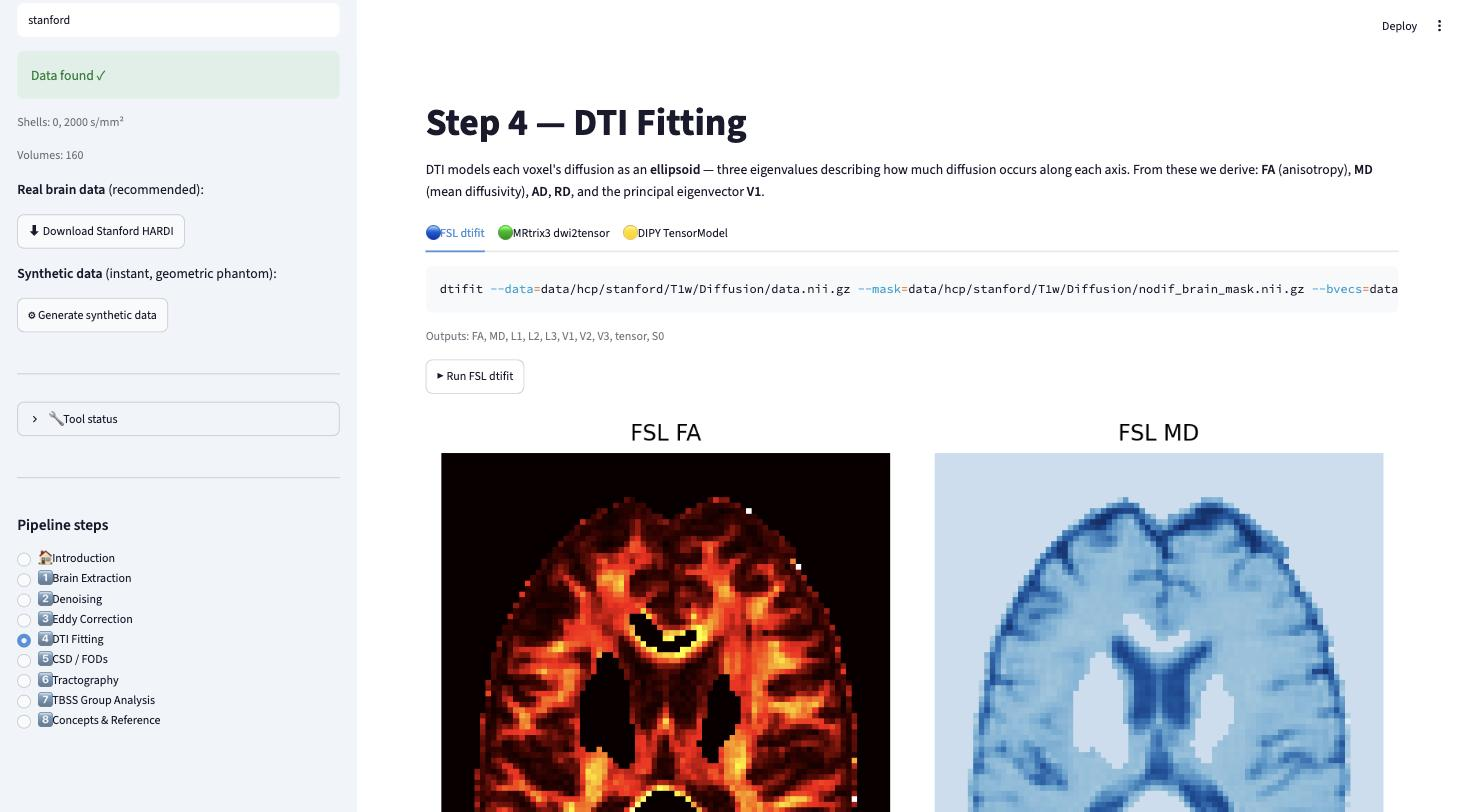
\includegraphics[width=1.0\textwidth]{figures/Figure2.png}
  \caption{The Stage 4 (DTI Fitting) user interface, representative of all seven pipeline stages, shown on the Stanford HARDI dataset. The sidebar (left) reports the resolved dataset --- detected shells and volume count --- and lists the eight pipeline pages; a collapsible Tool status panel reports which toolkit binaries are present in the current environment. The main panel presents three tabs, one per toolkit (FSL \texttt{dtifit}, MRtrix3 \texttt{dwi2tensor}, DIPY \texttt{TensorModel}). The selected tab shows the exact executable command with syntax highlighting, the outputs that command will produce, a Run button that submits it via Python \texttt{subprocess} and streams stdout and stderr live, and the resulting metric maps rendered below (FSL FA and MD shown here). The collapsible Why? section, further down the page, provides biological and mathematical context and guidance on when to prefer the current toolkit.}
  \label{fig:Figure2}
\end{figure}



\subsection{Runtime Performance}\label{runtime-performance}

On standard laptop hardware (macOS 14, Apple M2, 16 GB RAM; Docker Desktop, 8 GB memory allocation), all pipeline stages except eddy correction complete in under 3 minutes on the full 160-volume Stanford HARDI dataset. Eddy correction with FSL \texttt{eddy\_cpu} on the full dataset requires approximately 35--45 minutes on a single CPU core. The demo subsample mode (20 volumes) reduces this to approximately 2--4 minutes while preserving the educational content of the stage.

\section{Discussion}\label{discussion}

\subsection{Educational Contribution}\label{educational-contribution}

dMRI Rosetta Stone fills a specific gap in the neuroimaging training landscape that the comparison in Table 2 makes concrete. The closest existing analogue --- Andy's Brain Book (Jahn, 2020) --- covers FSL comprehensively and touches on MRtrix3, but is a read-only web resource with no code execution. DIPY tutorials are executable via Jupyter notebooks but cover DIPY exclusively. No existing resource places all three toolkits side by side on the same data in an executable format.

The Rosetta Stone metaphor is pedagogically productive. Learners with expertise in one toolkit can rapidly orient themselves in the syntax of another by reading the parallel tabs. Critically, the platform makes the \emph{asymmetries} as visible as the equivalences: the absence of CSD in FSL, the fact that \texttt{dwifslpreproc} delegates eddy correction to FSL \texttt{eddy} rather than implementing it independently, and the conceptually distinct tractography models (iFOD2 probabilistic in MRtrix3, deterministic DTI-peaks in DIPY, ROI-seeded probabilistic in FSL \texttt{probtrackx2}) are each highlighted explicitly with a contextual explanation.

Containerised deployment is especially valuable in workshop contexts. Organisers can distribute the Docker image to participants in advance, eliminating the dependency installation bottlenecks that typically consume significant hands-on session time. The application runs on standard laptop hardware without GPU acceleration and has been tested on Linux (Ubuntu 22.04), macOS 13--14, and Windows 11 via Docker Desktop.

\subsection{Methodological Transparency and Reproducibility}\label{methodological-transparency-and-reproducibility}

dMRI Rosetta Stone contributes to methodological transparency at two levels. At the surface level, it makes implementation differences between toolkits visible and discussable: that FSL \texttt{eddy\_cpu} corrects eddy current distortions, signal dropout, and outlier replacement in addition to head motion, whereas DIPY \texttt{motion\_correction} performs rigid-body registration only, is a distinction that is rarely stated explicitly in published methods sections but is immediately apparent in the side-by-side interface. Similarly, the absence of CSD in FSL --- a non-trivial limitation for acquisitions with crossing fibres --- is not always communicated to students trained exclusively in FSL.

At a deeper level, the quantitative inter-tool agreement analysis presented here tests a proposition that is widely assumed but rarely demonstrated: that FSL, MRtrix3, and DIPY produce effectively interchangeable DTI scalar metrics when applied to the same data under controlled conditions. Our results support that proposition only in part, and the qualification is the more interesting half of the finding.

For MRtrix3 and DIPY the assumption holds comfortably, and it holds on both acquisitions. Agreement of r = 0.9990 and 0.9966 for FA, and r = 0.9965 and 0.9991 for MD, with limits of agreement an order of magnitude narrower than within-tract biological variability, means that a study analysed in one of these toolkits could have been analysed in the other with no material change to its tensor-derived results.

For FSL the assumption does not hold in the form usually assumed, and our two-dataset design is what makes this visible. Had we analysed the Stanford data alone, we would have reported a systematic offset of approximately 4\% in FA and 5\% in MD and concluded that a fixed, characterisable bias separates FSL from the other two. The Sherbrooke replication refutes that reading. The MD offset persists in direction but quadruples in magnitude, and the FA offset reverses sign entirely --- FSL FA is lower than MRtrix3 and DIPY on one acquisition and higher on the other.

The practical consequence is worse than a fixed bias would be. A constant offset is a nuisance parameter: once measured, it can be corrected, or absorbed into a covariate, or simply acknowledged. An offset whose sign depends on the acquisition is not correctable in that way, because there is nothing stable to correct for. An analyst pooling FA values across studies processed with different software cannot anticipate even the direction of the discrepancy, let alone its size, without re-running the comparison on their own data --- which is precisely what this platform makes cheap to do.

Two qualifications keep this in proportion. Within a single study processed consistently, the offset displaces every subject in the same direction and is therefore unlikely to manufacture a spurious group difference; the risk lies in cross-study and multi-site comparison, in normative reference ranges, and in meta-analyses of absolute diffusivity. And toolkit choice at the tensor-fitting stage remains a smaller source of variance than acquisition protocol or preprocessing. But ``smaller'' is not ``negligible'', and an effect that changes sign between two ordinary open datasets is not one that a methods section can responsibly leave unstated. The asymmetry we observe --- two toolkits agreeing almost exactly while the third diverges unpredictably from both --- is exactly the kind of implementation-level behaviour that side-by-side execution exposes and that reading three sets of documentation does not.

However, the shell selection asymmetry identified in Stage 4 --- FSL and MRtrix3 including all shells by default while DIPY is explicit --- serves as a concrete example of where implementation differences \emph{do} matter for multi-shell data. This asymmetry is not captured by any existing documentation comparison but is immediately apparent in the dMRI Rosetta Stone interface. Several studies have demonstrated that such pipeline-level choices introduce non-trivial variability in dMRI-derived metrics (Bhagwat et al., 2021; Richie-Halford et al., 2022); the present platform makes this variability directly observable and educationally exploitable rather than merely reported.

\subsection{Comparison with Existing Resources}\label{comparison-with-existing-resources}

\begin{table}[H]
\caption*{\textbf{Table 2. Comparison of dMRI Rosetta Stone with existing dMRI educational resources.}}
\centering\footnotesize
\hyphenpenalty=10000\exhyphenpenalty=10000\relax
\begin{tabular}{@{}
  >{\raggedright\arraybackslash}p{(\linewidth - 10\tabcolsep) * \real{0.1667}}
  >{\raggedright\arraybackslash}p{(\linewidth - 10\tabcolsep) * \real{0.1667}}
  >{\raggedright\arraybackslash}p{(\linewidth - 10\tabcolsep) * \real{0.1667}}
  >{\raggedright\arraybackslash}p{(\linewidth - 10\tabcolsep) * \real{0.1667}}
  >{\raggedright\arraybackslash}p{(\linewidth - 10\tabcolsep) * \real{0.1667}}
  >{\raggedright\arraybackslash}p{(\linewidth - 10\tabcolsep) * \real{0.1667}}@{}}
\toprule
\begin{minipage}[b]{\linewidth}\raggedright
Resource
\end{minipage} & \begin{minipage}[b]{\linewidth}\raggedright
Toolkits
\end{minipage} & \begin{minipage}[b]{\linewidth}\raggedright
Executable
\end{minipage} & \begin{minipage}[b]{\linewidth}\raggedright
Real human data
\end{minipage} & \begin{minipage}[b]{\linewidth}\raggedright
Cross-tool, side-by-side
\end{minipage} & \begin{minipage}[b]{\linewidth}\raggedright
No local install
\end{minipage} \\
\midrule

\bottomrule

FSL Course / wiki & FSL & Local FSL required & Yes & No & No \\
MRtrix3 documentation & MRtrix3 & Local MRtrix3 required & Example data & No & No \\
DIPY tutorials & DIPY & Yes (Jupyter) & Yes & No & No (Python) \\
Andy's Brain Book (Jahn, 2020) & FSL, some MRtrix3 & No (read-only) & Screenshots & Partial, manual & No \\
NeuroHackademy recordings & Multiple & No (video) & Screenshots & No & No \\
Brainlife.io & Multiple & Yes (cloud) & Yes & No & No (account) \\
\textbf{dMRI Rosetta Stone} & \textbf{FSL + MRtrix3 + DIPY} & \textbf{Yes (Docker)} & \textbf{Yes} & \textbf{Yes} & \textbf{Docker only} \\
\end{tabular}
\end{table}

The only dimension on which dMRI Rosetta Stone is not strictly superior to all alternatives is that it requires a Docker installation and the project image (see Limitations for its size) rather than being fully browser-native. Docker is currently necessary to bundle FSL and MRtrix3, which do not support WebAssembly compilation. Future work may remove this barrier.

Brainlife.io warrants a specific note. It is a cloud-based provenance-tracking and pipeline-execution platform that supports multiple neuroimaging tools, including FSL and MRtrix3 applications (Avesani et al., 2019). Its purpose is fundamentally different from dMRI Rosetta Stone: users upload their own research data, select a pre-packaged application, and run it on cloud infrastructure to obtain results with full provenance records. Brainlife.io does not provide tutorial scaffolding, side-by-side command comparison, or the conceptual explanation layer that learners need to understand what each operation does and why. It is designed for reproducible research execution, not for cross-tool education.

\subsection{Scalability}\label{scalability}

The platform and the benchmark scale differently, and it is worth separating them.

The interactive application is deliberately single-subject and single-machine. Each pipeline stage runs one command on one dataset in a container sized for a laptop, because its purpose is comprehension rather than throughput: a learner needs to see one operation clearly, not to process a cohort. Within that scope it scales adequately. All stages except eddy correction complete in under three minutes on the full 160-volume Stanford acquisition on an Apple M2 with 8 GB allocated to Docker; eddy correction is the single bottleneck at 35--45 minutes on one CPU core, which the demo subsample mode reduces to 2--4 minutes for teaching purposes. Memory scales with volume count and matrix size, and the largest dataset used here (Sherbrooke, 193 volumes at 128 $\times$ 128 $\times$ 60) ran comfortably within the same allocation. The platform is explicitly not a cohort-processing pipeline, and users with that requirement should reach for a purpose-built workflow such as QSIPrep or a Nipype-based pipeline; nothing in this platform competes with those, and the Concepts and Reference module says so.

The benchmark scripts scale further, and were designed to. Adding a dataset requires one fetcher entry and two commands, which is how the Sherbrooke replication was produced; outputs are written per subject so that datasets accumulate rather than overwrite one another, and the \texttt{-\/-shell} option makes multi-shell acquisitions tractable without hand-editing gradient tables. The cost per dataset is one tensor fit per toolkit, which is minutes rather than hours. This matters for the finding reported above: establishing how the FSL divergence depends on acquisition would require tens of datasets rather than two, and that is a matter of compute time and data access rather than of software redesign. We regard extending this benchmark as the most valuable use of the codebase beyond teaching.

The principal barrier to scale is not computational but distributional --- the container is large, and the following section addresses that.

\subsection{Limitations}\label{limitations}

The platform currently supports single-subject analysis only; multi-subject group analysis beyond the synthetic TBSS demonstration requires real group data not included in the repository. The demo subsample mode for eddy correction is not suitable for quantitative analysis. The Docker image occupies approximately 17.6 GB uncompressed (approximately 5.6 GB as distributed layers) and requires approximately 15 minutes to build, which may be prohibitive in low-bandwidth settings; a pre-built image on a public container registry would mitigate this. GPU-accelerated MRtrix3 operations are not available in the current CPU-only Docker configuration.

The inter-tool benchmark reported here carries its own limitations, and they bound what may be concluded from the FSL divergence we describe. It rests on one subject from each of two datasets. Two acquisitions are enough to demonstrate that the FSL discrepancy is not a fixed, correctable bias --- a single dataset would have suggested exactly the opposite --- but they are not enough to characterise how it varies, to attribute it to specific acquisition properties such as b-value, SNR, or the number of b = 0 volumes, or to place a confidence interval around it. The benchmark isolates the tensor-fitting stage deliberately, applying no denoising or eddy-current correction, so the numbers characterise one pipeline step rather than an end-to-end analysis; whether the divergence persists, grows, or is absorbed after realistic preprocessing is untested. It compares only FA and MD under each toolkit's default weighted-least-squares configuration, and each toolkit exposes fitting options that were not explored. Establishing how the FSL divergence depends on acquisition, and identifying its algorithmic origin, would require a dedicated multi-subject study spanning several protocols --- work that this platform is well suited to support but does not itself constitute.

Finally, the platform has not yet been evaluated in a formal user study; a structured assessment of learning outcomes in a workshop setting would strengthen the evidence base for its educational value.

\subsection{Future Directions}\label{future-directions}

Planned developments include: (i) cloud deployment (e.g., Binder or Google Colab) to support GPU-accelerated tractography without local Docker installation; (ii) extension to advanced modules including fixel-based analysis, NODDI modelling, and automated tract segmentation; (iii) support for real multi-subject datasets from OpenNeuro; and (iv) a structured workshop pilot with pre/post knowledge assessment.

\section{Conclusion}\label{conclusion}

dMRI Rosetta Stone is an open-source, containerised, interactive platform that enables side-by-side comparison, execution, and visual inspection of the complete dMRI preprocessing and analysis pipeline across FSL, MRtrix3, and DIPY. By running real human brain data through all three toolkits in a unified browser interface, the platform makes cross-tool translation immediately accessible to students and researchers at all levels of experience. The application addresses a genuine and previously unmet gap in the neuroimaging training landscape, and is designed to accelerate dMRI education while promoting the methodological transparency that reproducible neuroimaging science requires.

\section{Data Availability Statement}\label{data-availability-statement}

The complete source code, Dockerfile, and documentation are openly available at https://github.com/happybrotherhood/dmri-rosetta-stone under an MIT licence. The exact version reported here is archived on Zenodo as v1.0.0, doi:10.5281/zenodo.22106455; the concept DOI doi:10.5281/zenodo.22106454 always resolves to the most recent version. Both demonstration datasets --- Stanford HARDI and Sherbrooke 3-shell --- are distributed openly by the DIPY project at https://dipy.org and are retrieved automatically by \texttt{scripts/fetch\_sample\_data.py}. No registration or credentials are required to reproduce any result presented here, and the four commands that regenerate every reported value are given at the end of the Materials and Methods.

\section{Author Contributions}\label{author-contributions}

BM: Conceptualization, Data curation, Formal analysis, Methodology, Software, Validation, Visualization, Writing -- original draft, Writing -- review and editing.

\section{Funding}\label{funding}

{[}\emph{Complete before submission: include grant numbers and funding bodies.}{]}

\section{Conflict of Interest Statement}\label{conflict-of-interest-statement}

The author declares that the research was conducted in the absence of any commercial or financial relationships that could be construed as a potential conflict of interest.

\section{Acknowledgements}\label{acknowledgements}

{[}\emph{Complete before submission: supervisors, HPC resources, collaborators.}{]}

\section{References}\label{references}

Avesani P, McPherson B, Hayashi S, Caiafa CF, Henschel R, Garyfallidis E, et al.~(2019) The open diffusion data derivatives, brain data upcycling via integrated collection and reuse. \emph{Scientific Data} 6, 69. doi: 10.1038/s41597-019-0073-y

Andersson JLR and Sotiropoulos SN (2016) An integrated approach to correction for off-resonance effects and subject movement in diffusion MR imaging. \emph{NeuroImage} 125, 1063--1078. doi: 10.1016/j.neuroimage.2015.10.019

Basser PJ, Mattiello J, and LeBihan D (1994) MR diffusion tensor spectroscopy and imaging. \emph{Biophysical Journal} 66, 259--267. doi: 10.1016/S0006-3495(94)80775-1

Beaulieu C (2002) The basis of anisotropic water diffusion in the nervous system -- a technical review. \emph{NMR in Biomedicine} 15, 435--455. doi: 10.1002/nbm.782

Bhagwat N, Barry A, Dickie EW, Brown ST, Devenyi GA, Hatano K, et al.~(2021) Understanding the impact of preprocessing pipelines on neuroimaging cortical surface analyses. \emph{GigaScience} 10, giaa155. doi: 10.1093/gigascience/giaa155

Catani M and Thiebaut de Schotten M (2008) A diffusion tensor imaging tractography atlas for virtual in vivo dissections. \emph{Cortex} 44, 1105--1132. doi: 10.1016/j.cortex.2008.05.004

Garyfallidis E, Brett M, Amirbekian B, Rokem A, Van Der Walt S, Descoteaux M, et al.~(2014) Dipy, a library for the analysis of diffusion MRI data. \emph{Frontiers in Neuroinformatics} 8, 8. doi: 10.3389/fninf.2014.00008

Glasser MF, Sotiropoulos SN, Wilson JA, Coalson TS, Fischl B, Andersson JL, et al.~(2013) The minimal preprocessing pipelines for the Human Connectome Project. \emph{NeuroImage} 80, 105--124. doi: 10.1016/j.neuroimage.2013.04.127

Jahn A (2020) \emph{Andy's Brain Book: An Introduction to Neuroimaging Analysis}. Available at: https://andysbrainbook.readthedocs.io (Accessed June 2026).

Jenkinson M, Beckmann CF, Behrens TEJ, Woolrich MW, and Smith SM (2012) FSL. \emph{NeuroImage} 62, 782--790. doi: 10.1016/j.neuroimage.2011.09.015

Jeurissen B, Tournier JD, Dhollander T, Connelly A, and Sijbers J (2014) Multi-tissue constrained spherical deconvolution for improved analysis of multi-shell diffusion MRI data. \emph{NeuroImage} 103, 411--426. doi: 10.1016/j.neuroimage.2014.07.061

Jones DK (ed.) (2010) \emph{Diffusion MRI: Theory, Methods, and Applications}. Oxford: Oxford University Press.

Merkel D (2014) Docker: Lightweight Linux containers for consistent development and deployment. \emph{Linux Journal} 2014, 2.

Richie-Halford A, Cieslak M, Ai L, Caffarra S, Covitz S, Franco AR, et al.~(2022) An analysis-ready and quality controlled resource for pediatric brain white-matter research. \emph{Scientific Data} 9, 616. doi: 10.1038/s41597-022-01695-7

Rokem A, Yeatman JD, Pestilli F, Kay KN, Mezer A, van der Walt S, et al.~(2015) Evaluating the accuracy of diffusion MRI models in white matter. \emph{PLOS ONE} 10, e0123272. doi: 10.1371/journal.pone.0123272

Smith RE, Tournier JD, Calamante F, and Connelly A (2015) SIFT2: Enabling dense quantitative assessment of brain white matter connectivity using streamlines tractography. \emph{NeuroImage} 119, 338--351. doi: 10.1016/j.neuroimage.2015.06.092

Smith SM, Jenkinson M, Woolrich MW, Beckmann CF, Behrens TEJ, Johansen-Berg H, et al.~(2004) Advances in functional and structural MR image analysis and implementation as FSL. \emph{NeuroImage} 23 (Suppl 1), S208--S219. doi: 10.1016/j.neuroimage.2004.07.051

Smith SM, Jenkinson M, Johansen-Berg H, Rueckert D, Nichols TE, Mackay CE, et al.~(2006) Tract-based spatial statistics: Voxelwise analysis of multi-subject diffusion data. \emph{NeuroImage} 31, 1487--1505. doi: 10.1016/j.neuroimage.2006.02.024

Streamlit Inc (2019) \emph{Streamlit: The fastest way to build and share data apps} {[}Computer software{]}. Available at: https://streamlit.io

Tournier JD, Calamante F, and Connelly A (2007) Robust determination of the fibre orientation distribution in diffusion MRI: Non-negativity constrained super-resolved spherical deconvolution. \emph{NeuroImage} 35, 1459--1472. doi: 10.1016/j.neuroimage.2007.02.016

Tournier JD, Calamante F, and Connelly A (2010) Improved probabilistic streamlines tractography by 2nd order integration over fibre orientation distributions. \emph{Proceedings of the International Society for Magnetic Resonance in Medicine} 18, 1670.

Tournier JD, Smith RE, Raffelt D, Tabbara R, Dhollander T, Pietsch M, et al.~(2019) MRtrix3: A fast, flexible and open software framework for medical image processing and visualisation. \emph{NeuroImage} 202, 116137. doi: 10.1016/j.neuroimage.2019.116137

Van Essen DC, Smith SM, Barch DM, Behrens TEJ, Yacoub E, Ugurbil K, et al.~(2013) The WU-Minn Human Connectome Project: An overview. \emph{NeuroImage} 80, 62--79. doi: 10.1016/j.neuroimage.2013.05.041

Veraart J, Novikov DS, Christiaens D, Ades-aron B, Sijbers J, and Fieremans E (2016) Denoising of diffusion MRI using random matrix theory. \emph{NeuroImage} 142, 394--406. doi: 10.1016/j.neuroimage.2016.08.016

\section{Tables}\label{tables}

\begin{table}[H]
\caption*{\textbf{Table 1. Pipeline stage coverage across FSL, MRtrix3, and DIPY in dMRI Rosetta Stone.} Dashes indicate the toolkit does not provide a dedicated implementation for that operation.}
\centering\footnotesize
\hyphenpenalty=10000\exhyphenpenalty=10000\relax
\begin{tabular}{@{}
  >{\raggedright\arraybackslash}p{(\linewidth - 8\tabcolsep) * \real{0.2000}}
  >{\raggedright\arraybackslash}p{(\linewidth - 8\tabcolsep) * \real{0.2000}}
  >{\raggedright\arraybackslash}p{(\linewidth - 8\tabcolsep) * \real{0.2000}}
  >{\raggedright\arraybackslash}p{(\linewidth - 8\tabcolsep) * \real{0.2000}}
  >{\raggedright\arraybackslash}p{(\linewidth - 8\tabcolsep) * \real{0.2000}}@{}}
\toprule
\begin{minipage}[b]{\linewidth}\raggedright
Stage
\end{minipage} & \begin{minipage}[b]{\linewidth}\raggedright
Operation
\end{minipage} & \begin{minipage}[b]{\linewidth}\raggedright
FSL
\end{minipage} & \begin{minipage}[b]{\linewidth}\raggedright
MRtrix3
\end{minipage} & \begin{minipage}[b]{\linewidth}\raggedright
DIPY
\end{minipage} \\
\midrule

\bottomrule

1 & Brain extraction & \texttt{bet} & \texttt{dwi2mask} & \texttt{median\_otsu} \\
2 & Denoising (MP-PCA) & --- & \texttt{dwidenoise} & \texttt{mppca} \\
3 & Eddy and motion correction & \texttt{eddy\_cpu} & \texttt{dwifslpreproc} & \texttt{motion\_correction} \\
4 & DTI fitting & \texttt{dtifit} & \texttt{dwi2tensor} + \texttt{tensor2metric} & \texttt{TensorModel} \\
5 & CSD / fibre orientation distributions & --- & \texttt{dwi2fod} (msmt-CSD) & \texttt{ConstrainedSphericalDeconvModel} \\
6 & Tractography & \texttt{probtrackx2} & \texttt{tckgen} (iFOD2) + \texttt{tcksift2} & \texttt{LocalTracking} \\
7 & Voxelwise group analysis & \texttt{tbss\_1–4} + \texttt{randomise} & --- & --- \\
\end{tabular}
\end{table}

\begin{table}[H]
\caption*{\textbf{Table 3. Quantitative inter-tool agreement for brain masks and DTI scalar metrics, on two independent open datasets.} Brain mask agreement assessed by Dice similarity coefficient (DSC) between each pair of per-tool brain extractions. DTI metric agreement assessed over white matter voxels (FA \textgreater{} 0.2 in all three tools) by Pearson correlation coefficient (r), mean absolute error (MAE), Bland--Altman mean bias, and 95\% limits of agreement (LoA). All three tensor fits used the same shared brain mask and the same volume subset, so metric differences reflect tensor fitting rather than masking or shell selection. MD in \textmu{}m\textsuperscript{2}/ms. Statistics are restricted to voxels physically admissible in both tools of the pair (FA $\in$ {[}0, 1{]}; 0 \textless{} MD $\leq$ 3.0 $\times$ $10^{-3}$ mm\textsuperscript{2}/s); per-tool counts of excluded voxels are reported in Table 4. All values generated by \texttt{scripts/compute\_fa\_comparison.py}.}
\emph{Stanford HARDI (single shell, b = 2000 s/mm\textsuperscript{2}, 160 volumes; n = 65,002 white matter voxels)}\par\smallskip
\centering\footnotesize
\hyphenpenalty=10000\exhyphenpenalty=10000\relax
\begin{tabular}{@{}
  >{\raggedright\arraybackslash}p{(\linewidth - 14\tabcolsep) * \real{0.1250}}
  >{\raggedright\arraybackslash}p{(\linewidth - 14\tabcolsep) * \real{0.1250}}
  >{\raggedright\arraybackslash}p{(\linewidth - 14\tabcolsep) * \real{0.1250}}
  >{\raggedright\arraybackslash}p{(\linewidth - 14\tabcolsep) * \real{0.1250}}
  >{\raggedright\arraybackslash}p{(\linewidth - 14\tabcolsep) * \real{0.1250}}
  >{\raggedright\arraybackslash}p{(\linewidth - 14\tabcolsep) * \real{0.1250}}
  >{\raggedright\arraybackslash}p{(\linewidth - 14\tabcolsep) * \real{0.1250}}
  >{\raggedright\arraybackslash}p{(\linewidth - 14\tabcolsep) * \real{0.1250}}@{}}
\toprule
\begin{minipage}[b]{\linewidth}\raggedright
Comparison
\end{minipage} & \begin{minipage}[b]{\linewidth}\raggedright
Mask DSC
\end{minipage} & \begin{minipage}[b]{\linewidth}\raggedright
FA r
\end{minipage} & \begin{minipage}[b]{\linewidth}\raggedright
FA MAE
\end{minipage} & \begin{minipage}[b]{\linewidth}\raggedright
FA bias
\end{minipage} & \begin{minipage}[b]{\linewidth}\raggedright
FA 95\% LoA
\end{minipage} & \begin{minipage}[b]{\linewidth}\raggedright
MD r
\end{minipage} & \begin{minipage}[b]{\linewidth}\raggedright
MD MAE
\end{minipage} \\
\midrule

\bottomrule

FSL vs.~DIPY & 0.9277 & 0.9604 & 0.0228 & $-$0.0158 & {[}$-$0.0992, +0.0676{]} & 0.9368 & 0.0325 \\
FSL vs.~MRtrix3 & 0.9024 & 0.9652 & 0.0247 & $-$0.0181 & {[}$-$0.0964, +0.0602{]} & 0.9402 & 0.0333 \\
MRtrix3 vs.~DIPY & 0.9009 & 0.9990 & 0.0029 & +0.0027 & {[}$-$0.0107, +0.0162{]} & 0.9965 & 0.0012 \\
\end{tabular}
\end{table}

\emph{Sherbrooke 3-shell (b = 0 + b = 1000 s/mm\textsuperscript{2} subset, 65 volumes; n = 111,032 white matter voxels)}

\begin{table}[htbp]
\centering\footnotesize
\hyphenpenalty=10000\exhyphenpenalty=10000\relax
\begin{tabular}{@{}
  >{\raggedright\arraybackslash}p{(\linewidth - 14\tabcolsep) * \real{0.1250}}
  >{\raggedright\arraybackslash}p{(\linewidth - 14\tabcolsep) * \real{0.1250}}
  >{\raggedright\arraybackslash}p{(\linewidth - 14\tabcolsep) * \real{0.1250}}
  >{\raggedright\arraybackslash}p{(\linewidth - 14\tabcolsep) * \real{0.1250}}
  >{\raggedright\arraybackslash}p{(\linewidth - 14\tabcolsep) * \real{0.1250}}
  >{\raggedright\arraybackslash}p{(\linewidth - 14\tabcolsep) * \real{0.1250}}
  >{\raggedright\arraybackslash}p{(\linewidth - 14\tabcolsep) * \real{0.1250}}
  >{\raggedright\arraybackslash}p{(\linewidth - 14\tabcolsep) * \real{0.1250}}@{}}
\toprule
\begin{minipage}[b]{\linewidth}\raggedright
Comparison
\end{minipage} & \begin{minipage}[b]{\linewidth}\raggedright
Mask DSC
\end{minipage} & \begin{minipage}[b]{\linewidth}\raggedright
FA r
\end{minipage} & \begin{minipage}[b]{\linewidth}\raggedright
FA MAE
\end{minipage} & \begin{minipage}[b]{\linewidth}\raggedright
FA bias
\end{minipage} & \begin{minipage}[b]{\linewidth}\raggedright
FA 95\% LoA
\end{minipage} & \begin{minipage}[b]{\linewidth}\raggedright
MD r
\end{minipage} & \begin{minipage}[b]{\linewidth}\raggedright
MD MAE
\end{minipage} \\
\midrule

\bottomrule

FSL vs.~DIPY & 0.9668 & 0.8897 & 0.0504 & +0.0148 & {[}$-$0.1640, +0.1937{]} & 0.9012 & 0.1272 \\
FSL vs.~MRtrix3 & 0.9058 & 0.9157 & 0.0460 & +0.0139 & {[}$-$0.1419, +0.1696{]} & 0.9020 & 0.1271 \\
MRtrix3 vs.~DIPY & 0.9163 & 0.9966 & 0.0059 & +0.0053 & {[}$-$0.0260, +0.0366{]} & 0.9991 & 0.0029 \\
\end{tabular}
\end{table}

\begin{table}[H]
\caption*{\textbf{Table 4. Non-physical tensor fits within the white matter mask.} Counts of voxels violating the definition of each metric, with the percentage of the white matter mask in parentheses.}
\centering\footnotesize
\hyphenpenalty=10000\exhyphenpenalty=10000\relax
\begin{tabular}{@{}
  >{\raggedright\arraybackslash}p{(\linewidth - 8\tabcolsep) * \real{0.2000}}
  >{\raggedright\arraybackslash}p{(\linewidth - 8\tabcolsep) * \real{0.2000}}
  >{\raggedright\arraybackslash}p{(\linewidth - 8\tabcolsep) * \real{0.2000}}
  >{\raggedright\arraybackslash}p{(\linewidth - 8\tabcolsep) * \real{0.2000}}
  >{\raggedright\arraybackslash}p{(\linewidth - 8\tabcolsep) * \real{0.2000}}@{}}
\toprule
\begin{minipage}[b]{\linewidth}\raggedright
Dataset
\end{minipage} & \begin{minipage}[b]{\linewidth}\raggedright
Metric
\end{minipage} & \begin{minipage}[b]{\linewidth}\raggedright
FSL
\end{minipage} & \begin{minipage}[b]{\linewidth}\raggedright
MRtrix3
\end{minipage} & \begin{minipage}[b]{\linewidth}\raggedright
DIPY
\end{minipage} \\
\midrule

\bottomrule

Stanford (n = 65,002) & FA \textgreater{} 1 & 261 (0.40\%) & 178 (0.27\%) & 0 (0\%) \\
Stanford & MD $\leq$ 0 & 261 (0.40\%) & 91 (0.14\%) & 0 (0\%) \\
Sherbrooke (n = 111,032) & FA \textgreater{} 1 & 4,404 (3.97\%) & 2,252 (2.03\%) & 0 (0\%) \\
Sherbrooke & MD $\leq$ 0 & 3,016 (2.72\%) & 603 (0.54\%) & 0 (0\%) \\
\end{tabular}
\end{table}

\clearpage
\section*{Supplementary Figures}
\renewcommand{\thefigure}{S\arabic{figure}}
\setcounter{figure}{0}

\begin{figure}[tbp]
  \centering
  \setcounter{figure}{0}
  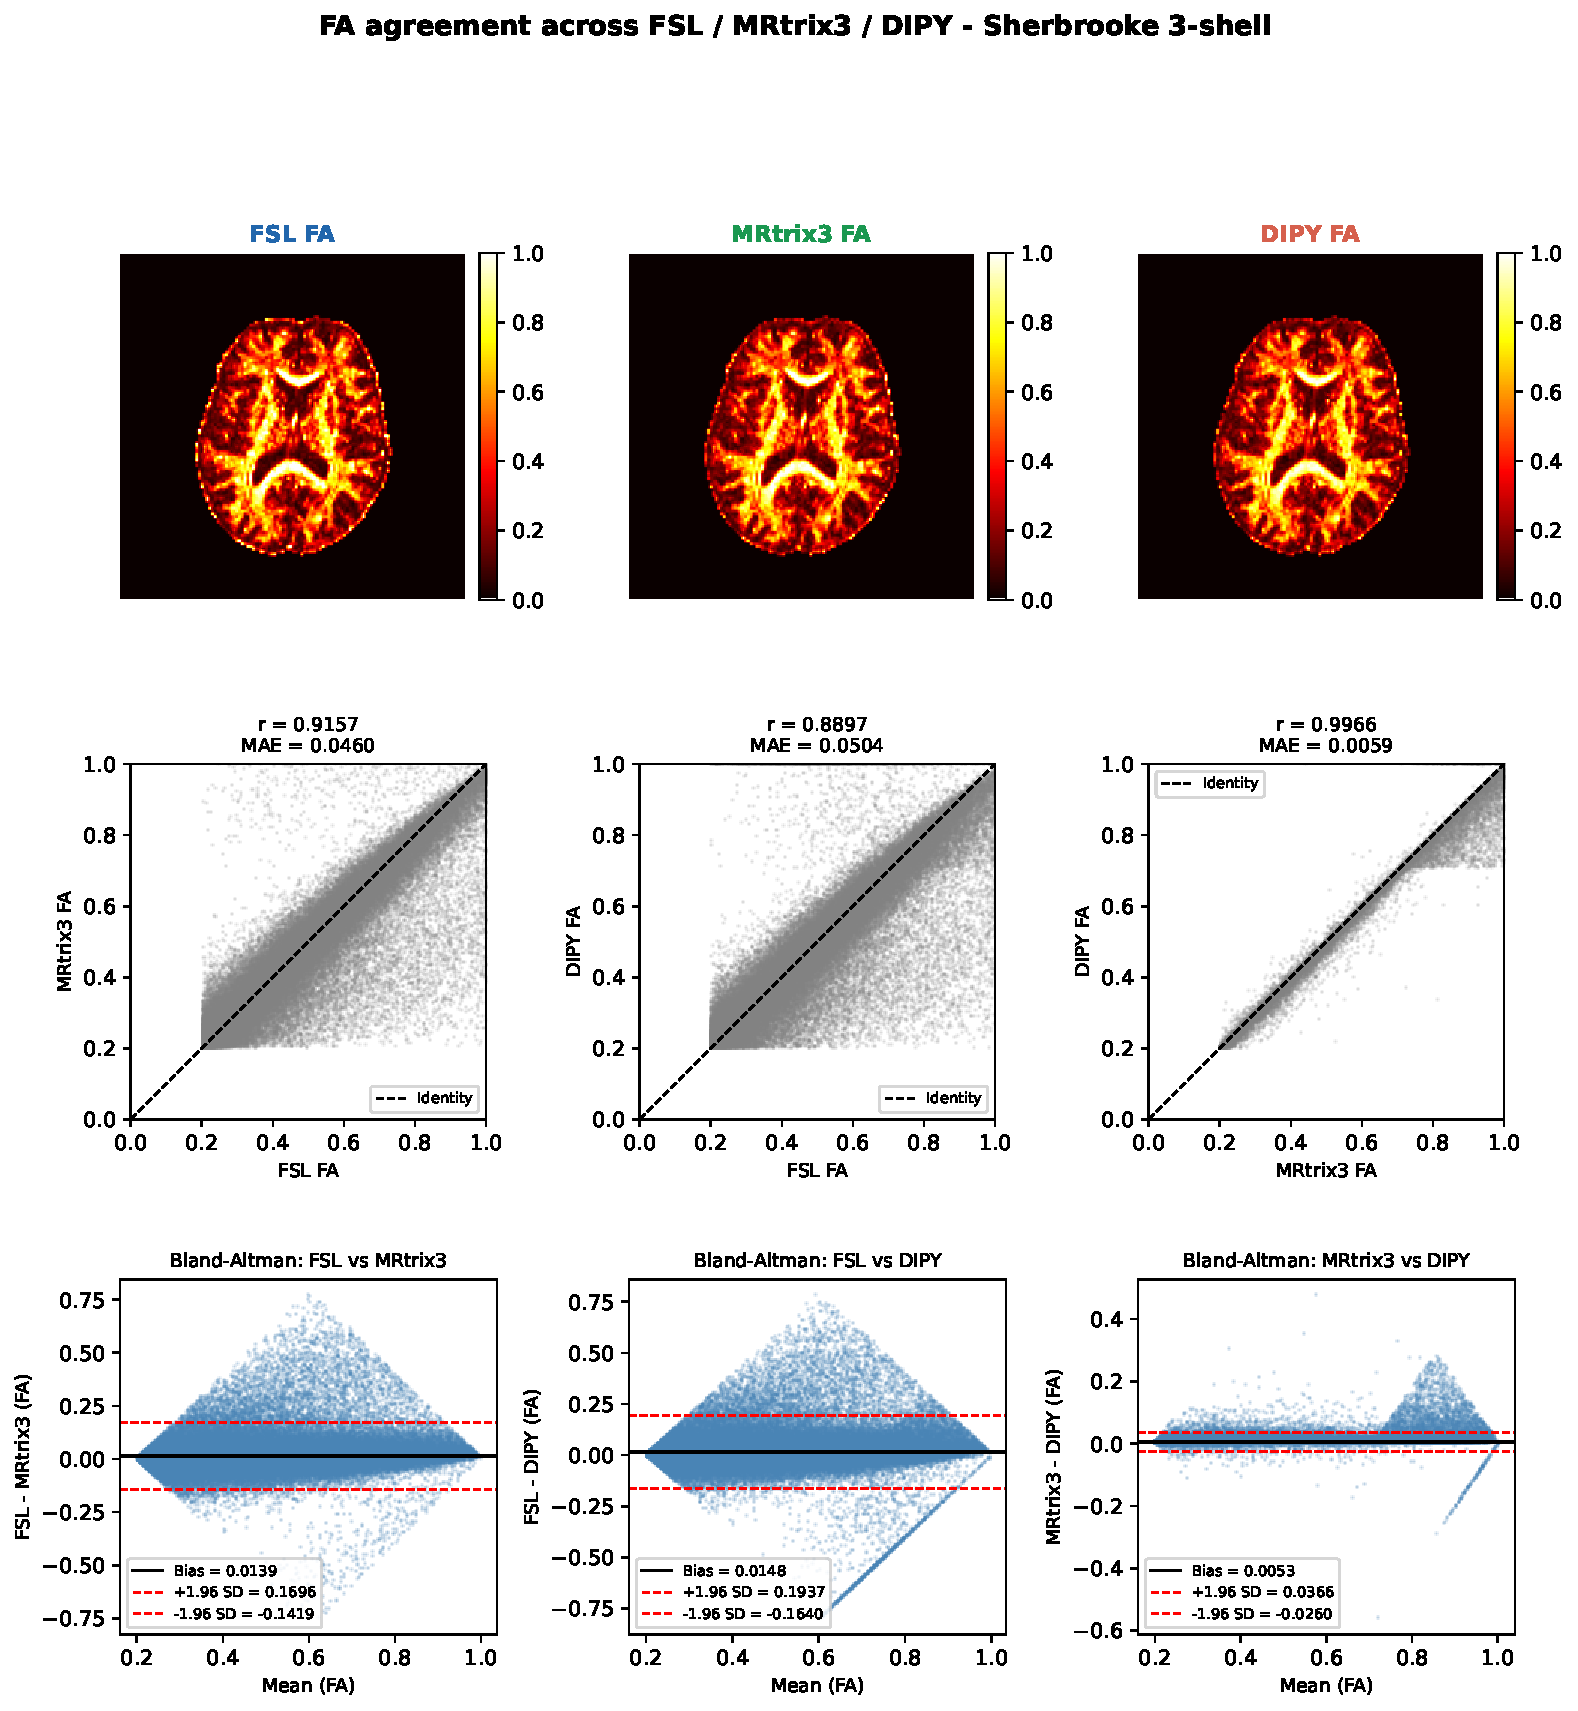
\includegraphics[width=0.86\textwidth]{figures/FigureS1.pdf}
  \caption{As Figure 3, for the Sherbrooke 3-shell dataset (b = 0 + b = 1000 s/mm\textsuperscript{2} subset).}
  \label{fig:FigureS1}
\end{figure}


\begin{figure}[tbp]
  \centering
  \setcounter{figure}{1}
  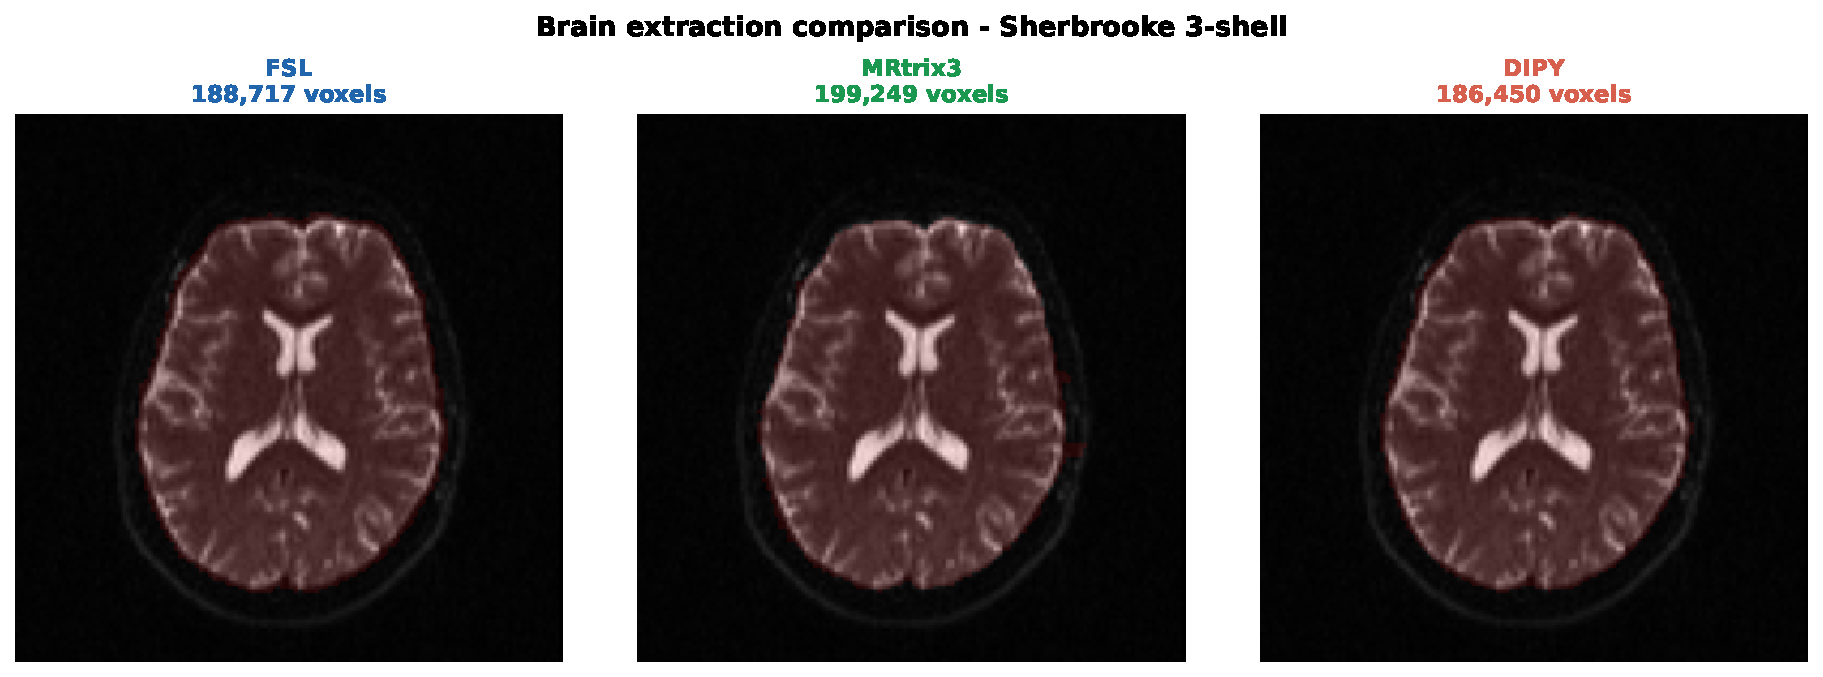
\includegraphics[width=1.0\textwidth]{figures/FigureS2.pdf}
  \caption{As Figure 4, for the Sherbrooke 3-shell dataset.}
  \label{fig:FigureS2}
\end{figure}


\end{document}
